\chapter{Event selection in ND-GAr}
\label{chapter:gar_selection}

\begin{chapquote}{Marcus Aurelius, \textit{Meditations}}
	You have power over your mind, not outside events. Realise this, and you will find strength.
\end{chapquote}

As discussed previously, it is necessary to evaluate the capabilities of ND-GAr at identifying different particles. In the context of the LBL analysis, we want ND-GAr to provide data samples containing events of specific topologies, like $\nu_{\mu}$ CC $1\pi^{\pm}$, $\nu_{\mu}$ CC $1p1\pi^{\pm}$, etcetera. Thus, developing a strategy for the event selection using the current reconstruction is required.

In this Chapter, I present the results of a number of preliminary studies focused on the event selection in ND-GAr, particularly the $\nu_{\mu}$ CC selection and the pion tagging strategies. I also investigate the neutrino energy reconstruction, as well as the systematic uncertainties relevant for our detector. The objective is to demonstrate that the assumptions made in the DUNE TDR are feasible with a full end-to-end ND GAr simulation. This means demonstrating that it is possible to reconstruct muon neutrino interactions, select pion exclusive samples, and measure relevant muon and pion quantities (including neutral pions).

\section{Simulated data sample}
\label{sec:gar_data}

For the event selection studies I produced a MC sample consisting of $10^{5}$ FHC neutrino interaction events inside the HPgTPC volume. The version of \texttt{GENIE} used was \texttt{v3_04_00}, with the \texttt{G18} configuration. This is a version of the re-tune produced from CCQE, CC$1\pi$, CC$2\pi$, and CC inclusive bubble chamber cross-section data \cite{GENIE2021}. It uses the local Fermi gas \cite{Chiang1989} as a description of the nuclear model. The quasielastic-like events are described by the Nieves quasielastic \cite{Nieves2004} and Valencia $2p2h$ \cite{Nieves2011} models. The Berger-Seghal model \cite{Berger2007,Berger2008} is used for the resonant and coherent pion production. As in all the \texttt{GENIE} tunes, the Bodek-Yang model \cite{Bodek2002} describes the DIS interactions. Finally, the FSI are described using the effective intranuclear transport model in INTRANUKE.

For this sample, I used \texttt{GArG4} instead of \texttt{edep-sim} for the particle propagation. Because both \texttt{Geant4} wrappers use different configurations for the simulation, the results obtained are different. The default \texttt{edep-sim} configuration used by the DUNE ND is appropriate for ND-LAr, where thresholds for particle production are higher. In the case of ND-GAr, these parameters need to be adjusted accordingly. For the time being, in these first productions of analysis files, we will use our standalone \texttt{Geant4} implementation.

The detector simulation and reconstruction used was GArSoft version \texttt{v02_21_00}. I made use of the standard routines for the readout simulation and the reconstruction, which include the additions described in section \ref{section:integration}. A summary of the GArSoft outputs is extracted in the form of a plain \texttt{ROOT} \texttt{TTree}. These are then used, together with the \texttt{GENIE} output files, to produce common analysis files (CAFs). The version of the CAF format used in this analysis is \texttt{duneanaobj} \texttt{v3_07_00}.

This sample only includes single interaction events. In the future, we will move to simulate full neutrino spills. Also, we will need to include neutrino interactions in the other detector volumes (ECal, magnet, \dots), as well as rock muons making it to ND-GAr. However, this will require a significant amount of work to go into the so-called interaction slicer, the part of the reconstruction in charge of splitting the reconstructed events.

\begin{table}[t]
	\caption[Estimated event rates in ND-GAr.]{Estimated event rates in ND-GAr, divided by interaction type and pion multiplicity, for two different values of the $\mathrm{POT}/\mathrm{year}$.}
	\begin{center}
		\begin{small}
			\begin{tabular}{lcc}
                & \multicolumn{2}{c}{Events/ton/year}                                                                   \\[2mm] \cline{2-3} 
            \multicolumn{1}{c}{\rule{0pt}{1.1\normalbaselineskip}Process}       & $1.1 \times 10^{21} ~ \mathrm{POT}/\mathrm{year}$ & $1.9 \times 10^{21} ~ \mathrm{POT}/\mathrm{year}$ \\[2mm] \hline
            \rule{0pt}{1.1\normalbaselineskip}All $\nu_{\mu}$-CC                & $1.60 \times 10^{6}$                              & $2.83 \times 10^{6}$                              \\[2mm]
            $\hspace{0.5 cm}$ CC $0\pi$       & $5.28 \times 10^{5}$                              & $9.35 \times 10^{5}$                              \\[2mm]
            $\hspace{0.5 cm}$ CC $1\pi^{\pm}$ & $3.02 \times 10^{5}$                              & $5.34 \times 10^{5}$                              \\[2mm]
            $\hspace{0.5 cm}$ CC $1\pi^{0}$   & $1.65 \times 10^{5}$                              & $2.92 \times 10^{5}$                              \\[2mm]
            $\hspace{0.5 cm}$ CC $2\pi$       & $3.18 \times 10^{5}$                              & $5.63 \times 10^{5}$                              \\[2mm]
            $\hspace{0.5 cm}$ CC $3\pi$       & $1.36 \times 10^{5}$                              & $2.41 \times 10^{5}$                              \\[2mm]
            $\hspace{0.5 cm}$ CC other        & $1.52 \times 10^{5}$                              & $2.69 \times 10^{5}$                              \\[2mm] \hline
            \rule{0pt}{1.1\normalbaselineskip}All $\bar{\nu}_{\mu}$-CC          & $7.54 \times 10^{4}$                              & $1.33 \times 10^{5}$                              \\[2mm]
            All NC                            & $5.50 \times 10^{5}$                              & $9.73 \times 10^{5}$                              \\[2mm]
            All $\nu_{e}$-CC                  & $2.70 \times 10^{4}$                              & $4.78 \times 10^{4}$                             
            \end{tabular}
		\end{small}
	\end{center}
	\label{tab:ndgar_event_rates}
\end{table}

Looking forward, these sort of small samples are useful to prepare before launching a full production of ND-GAr events. In the original DUNE TDR LBL analysis, the event rates are calculated with a $1.1 \times 10^{21} ~ \mathrm{POT}/\mathrm{year}$ assumption, which assumes a combined uptime and efficiency of the accelerator complex and the LBNF beamline of $57\%$ \cite{DUNE2020}. If we have one spill every $1.2~\mathrm{s}$, that translates into $7.5 \times 10^{13} ~ \mathrm{POT}/\mathrm{spill}$. Therefore, assuming that the POT/spill scales linearly with beam power, in Phase II we will have $1.3 \times 10^{14} ~ \mathrm{POT}/\mathrm{spill}$ for the for the $2.1 ~ \mathrm{MW}$ beam. Or equivalently, $1.9 \times 10^{21} ~ \mathrm{POT}/\mathrm{year}$ using the same efficiency. The event rates per year in ND-GAr computed for these two possible values of the POT/year are shown in Tab. \ref{tab:ndgar_event_rates}.

The latest PRISM plan requires $1.50 ~ \mathrm{POT} \cdot \mathrm{years}$ of data on-axis, followed by $0.25 ~ \mathrm{POT} \cdot \mathrm{years}$ at each off-axis position ($2$, $4$, $8$, $12$, $16$, $20$, $24$, and $28~\mathrm{m}$), both for FHC and RHC mode. This implies that a full on-axis ND-GAr production will require a total of $2.85 \times 10^{21}~\mathrm{POT}$ for both horn currents. The production of these samples is necessary to understand the impact of ND-GAr on the LBL sensitivities, and the studies presented here should be considered as a first step towards the realisation of such analysis.

\section[\texorpdfstring{$\nu_{\mu}$}{numu} CC selection]{\boldmath\texorpdfstring{$\nu_{\mu}$}{numu} CC selection}
\label{sec:gar_numu_cc}

In a $\nu_{\mu}$ CC inclusive selection, the signal topology we look for is a neutrino-induced muon with or without other final state particles. Here, I also require the neutrino vertex to be located inside the fiducial volume (FV) of ND-GAr.

The FV is defined as a smaller cylinder within the cylindrical volume of the HPgTPC. The FV has a radius $R_{\mathrm{FV}}$ and a half-length $L_{\mathrm{FV}}$. For a particle position to lie within the FV it must satisfy:
\begin{equation}
    \vec{x}_{i} \in \left\{\vec{x} \in \mathbb{R}^{3} \mid |x_{0}| \leq L_{\mathrm{FV}} ~ \& ~ \sqrt{x_{1}^{2}+x_{2}^{2}} \leq R_{\mathrm{FV}}\right\},
\end{equation}
in the reference frame of the HPgTPC. For convenience, I define:
\begin{equation}
    \begin{split}
        \Delta R_{\mathrm{FV}} &= R_{\mathrm{HPgTPC}} - R_{\mathrm{FV}}, \\
        \Delta L_{\mathrm{FV}} &= L_{\mathrm{HPgTPC}} - L_{\mathrm{FV}},
    \end{split}
\end{equation}
where $R_{\mathrm{HPgTPC}}$ and $L_{\mathrm{HPgTPC}}$ refer to the radius and the half-length of the HPgTPC, respectively. Figure \ref{fig:ndgar_ana_geometry} shows the HPgTPC volume with the FV inside of it. In that representation, the FV is defined as having $\Delta L_{\mathrm{FV}} = 30.0 ~ \mathrm{cm}$ and $\Delta R_{\mathrm{FV}} = 30.0 ~ \mathrm{cm}$. Also shown is the HPgTPC reference frame, with $x$ being the drift direction and $z$ aligned along the beam direction.

In some cases, it is interesting to divide the signal events in different categories based on their true interaction mode. In this work, I will distinguish between charged-current quasi-elastic (CCQE), meson exchange current (CCMEC), resonant (CCRES), and deep-inelastic (CCDIS) interactions. I also use a separate category for the interactions not included in any of the other categories (CCOther).

Any other events are considered backgrounds. For this selection, I use the following categorisation of background events:
\begin{itemize}
    \item Out of FV: if the true neutrino vertex lies outside the defined FV.
    \item NC: if the event is a true neutral-current event.
    \item $\bar{\nu}_{\mu}$ CC: if the true neutrino candidate is of muon antineutrino flavour.
    \item Other: if the event is not signal nor falls in any of the other background categories.
\end{itemize}

\begin{figure}[t]
\centering
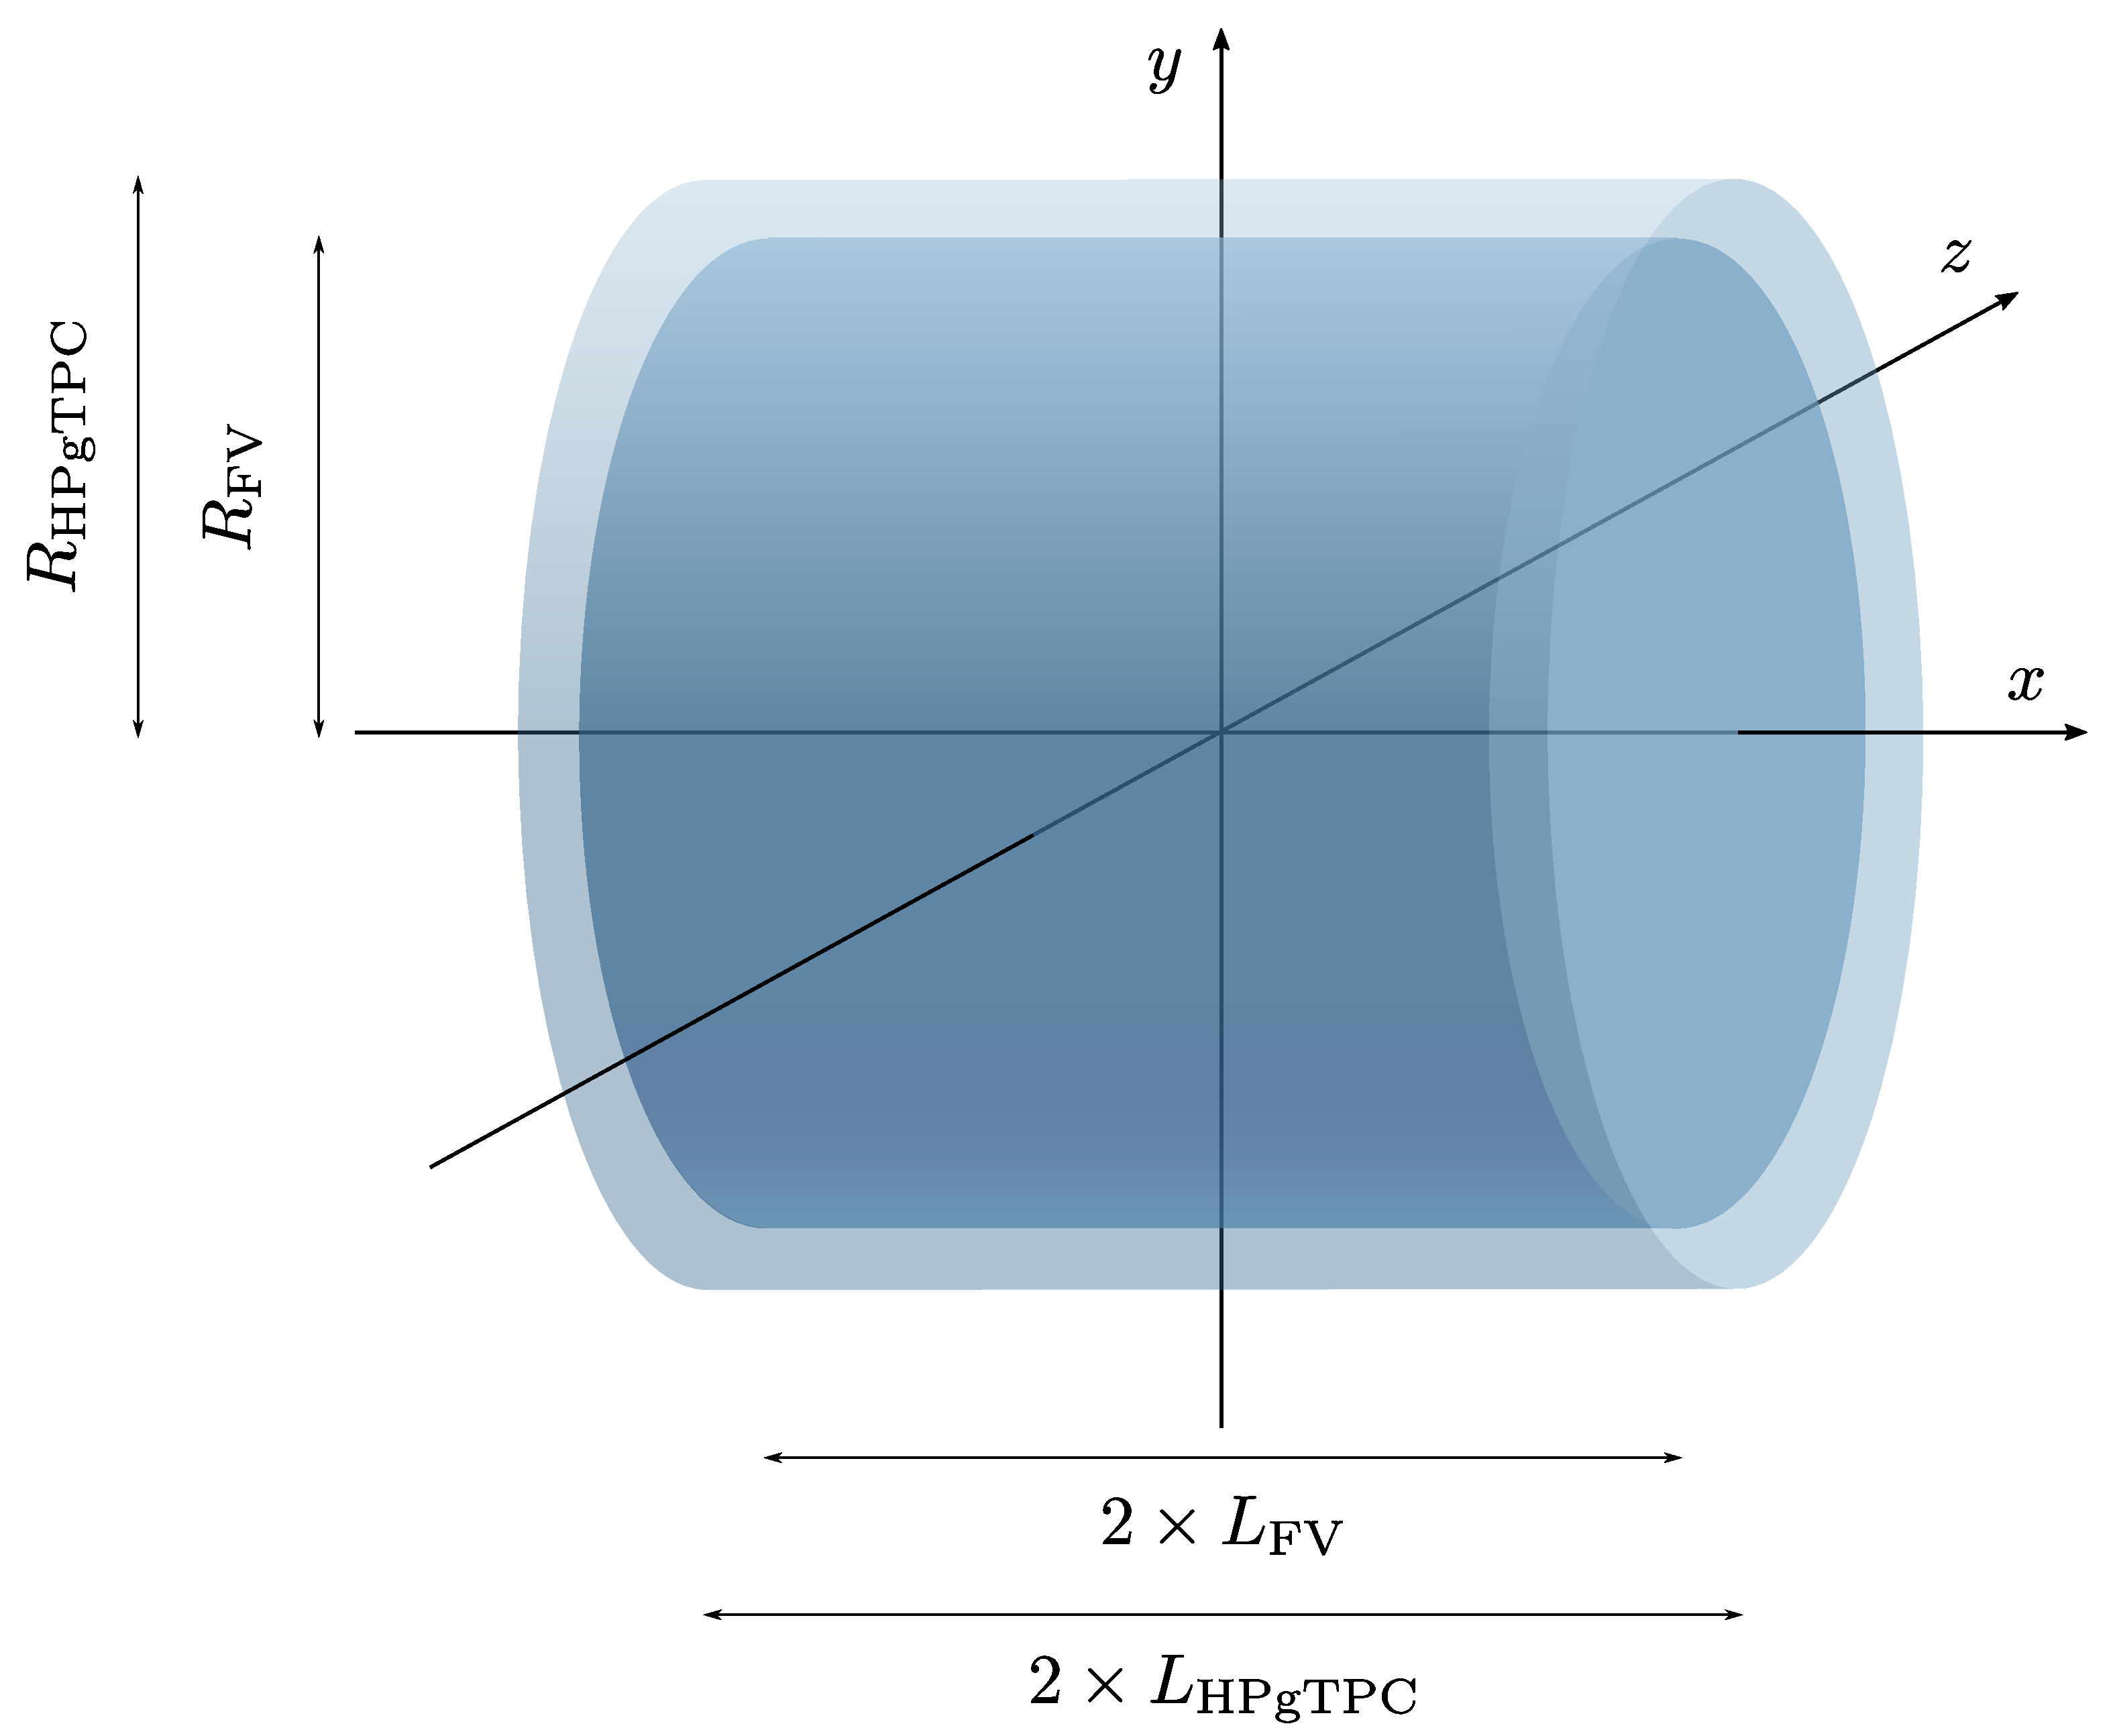
\includegraphics[width=.90\linewidth]{Images/GAr_selection/ndgar_ana_geometry.pdf}
\caption[Schematic diagram of the HPgTPC including the fiducial volume.]{Schematic diagram of the HPgTPC including the fiducial volume (FV). In this case the FV is given by $\Delta L_{\mathrm{FV}} = 30.0 ~ \mathrm{cm}$ and $\Delta R_{\mathrm{FV}} = 30.0 ~ \mathrm{cm}$.}
\label{fig:ndgar_ana_geometry}
\end{figure}

The key to the CC selection is the identification of a primary muon candidate. Typically, this is the longest track in the event. However, sometimes protons and pions leave tracks longer than that of the muon. This is particularly important in the GAr medium, considerably less dense than the LAr. For this reason, the muon identification in ND-GAr relies heavily on the capabilities of the ECal.

The selection strategy proposed combines the information coming from the three main detection systems of ND-GAr: the HPgTPC charge readout, and the ECal and $\mu$ID detectors. It consists of five steps:
\begin{enumerate}
    \item Event contains reconstructed particles.
    \item Select particles with reconstructed negative charge, $q_{\mathrm{reco}} = -1$.
    \item Select particles passing the muon score cut, $\mu_{\mathrm{score}} \geq \mu_{\mathrm{score}}^{\mathrm{cut}}$.
    \item Keep reconstructed particle with the highest momentum, $\mathrm{max}\left[p_{\mathrm{reco}}\right]$.
    \item Check that the remaining particle starts within the FV.
\end{enumerate}
All the events passing these cuts are classified as signal, and the selected particle is regarded as the primary muon candidate.

\begin{figure}[t]
    \centering
    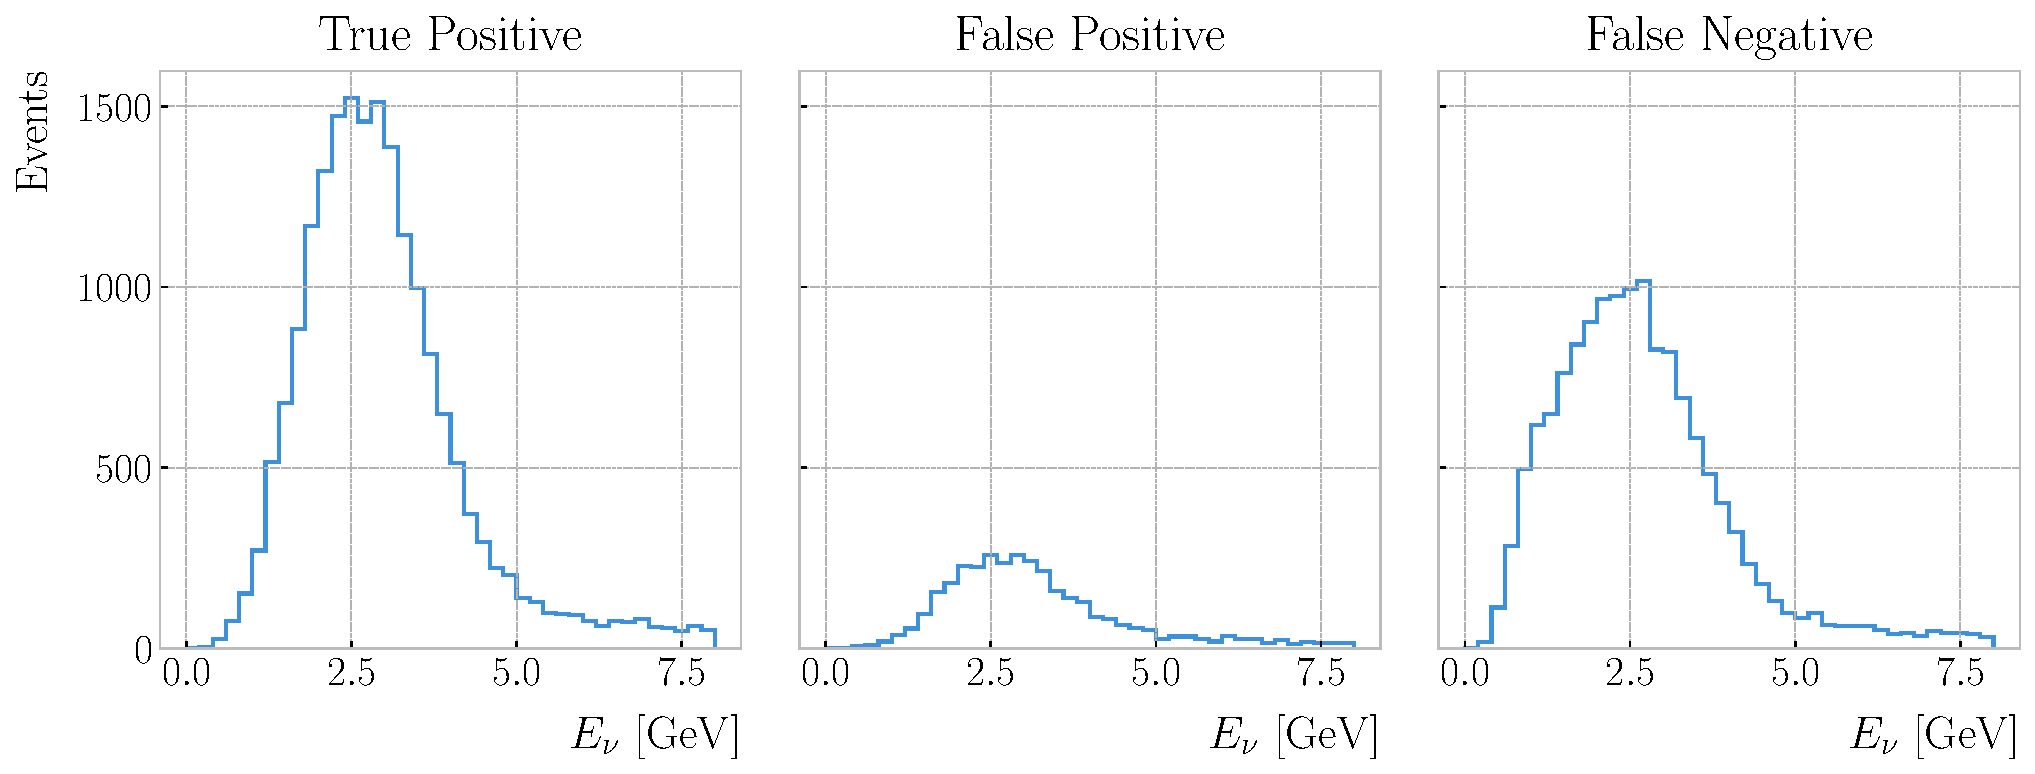
\includegraphics[width=.99\linewidth]{Images/GAr_selection/true_numu_example_spectra_horizontal.pdf}
    \caption[True positive, false positive, and false negative true neutrino energy distributions for a $\nu_{\mu}$ CC selection.]{True positive (left panel), false positive (middle panel), and false negative (right panel) true neutrino energy distributions for the $\nu_{\mu}$ CC selection given by a muon score cut of $\mu_{\mathrm{score}}^{\mathrm{cut}} = 0.75$, and a FV defined as $\Delta L_{\mathrm{FV}} = 30.0 ~ \mathrm{cm}$ and $\Delta R_{\mathrm{FV}} = 30.0 ~ \mathrm{cm}$.}
    \label{fig:numuCC_spectra_example}
\end{figure}

\subsection{Selection optimisation}

I performed an optimisation of this selection, comparing the performance of a number of configurations. For the muon selection, I varied the value of $\mu_{\mathrm{score}}^{\mathrm{cut}}$ from $0.05$ to $0.95$, using a step size of $0.05$. Additionally, to optimise the FV, I systematically explored a number of different parameter configurations, moving within the $10.0-70.0~\mathrm{cm}$ range for $\Delta L_{\mathrm{FV}}$ and $25.0-75.0~\mathrm{cm}$ for $\Delta R_{\mathrm{FV}}$, in increments of $10.0~\mathrm{cm}$ and $5.0~\mathrm{cm}$ respectively.

For each parameter configuration, I extract three different true neutrino energy distributions. These are built combining the results of the selection described previously, which we can refer to as the ``reco'' selection, and a ``true'' selection. The later identifies the true $\nu_{\mu}$ CC events using the GENIE event records, and checks that the true neutrino vertices are contained in the FV.

The first distribution consists of the events passing both selections, i.e., these are the true $\nu_{\mu}$ CC events which pass the ``reco'' selection. The second distribution contains the events passing the ``reco'' selection but failing the ``true'' selection. These are the background events that the selection misidentifies. Finally, the third distribution corresponds to the events picked by the ``true'' selection but not by the ``reco'' one. In other words, these are the true $\nu_{\mu}$ CC events that our selection misses. In analogy to the machine learning jargon, I refer to these distributions as the true positive (TP), false positive (FP), and false negative (FN) spectra, respectively. Figure \ref{fig:numuCC_spectra_example} shows an example of these three distributions for the case $\mu_{\mathrm{score}}^{\mathrm{cut}} = 0.75$, $\Delta L_{\mathrm{FV}} = 30.0 ~ \mathrm{cm}$, and $\Delta R_{\mathrm{FV}} = 30.0 ~ \mathrm{cm}$.

By making different combinations of these distributions one can compute a series of performance metrics. Using the full information from the spectra allows to obtain the scores as a function of the true neutrino energy, whereas the totals can be obtained by integrating the histograms. This way, the efficiency of the selection is given by:
\begin{equation}
    \begin{split}
        \mathrm{Efficiency} &= \frac{\text{Selected true } \nu_{\mu} \text{ CC events}}{\text{Total true } \nu_{\mu} \text{ CC events}}\\
        &= \frac{\mathrm{TP}}{\mathrm{TP}+\mathrm{FN}},
    \end{split}
\end{equation}
while the purity can be written as:
\begin{equation}
    \begin{split}
        \mathrm{Purity} &= \frac{\text{Selected true } \nu_{\mu} \text{ CC events}}{\text{Total selected events}}\\
        &= \frac{\mathrm{TP}}{\mathrm{TP}+\mathrm{FP}}.
    \end{split}
\end{equation}

Another scoring metric typically used when quantifying the performance of a selection is the significance. It is defined as:
\begin{equation}
    \mathrm{Significance} = \frac{S}{\sqrt{S+B}} = \frac{\mathrm{TP}}{\sqrt{\mathrm{TP} + \mathrm{FP}}}.
\end{equation}
The significance measures the relative size of the true signal within the selection, $S=\mathrm{TP}$ with respect to one standard deviation of the counting experiment. Assuming Poisson statistics, the variance is equal to the number of observations, and therefore the standard deviation equals to $\sqrt{N}=\sqrt{S+B}=\sqrt{\mathrm{TP} + \mathrm{FP}}$.

\begin{figure}[t]
    \centering
    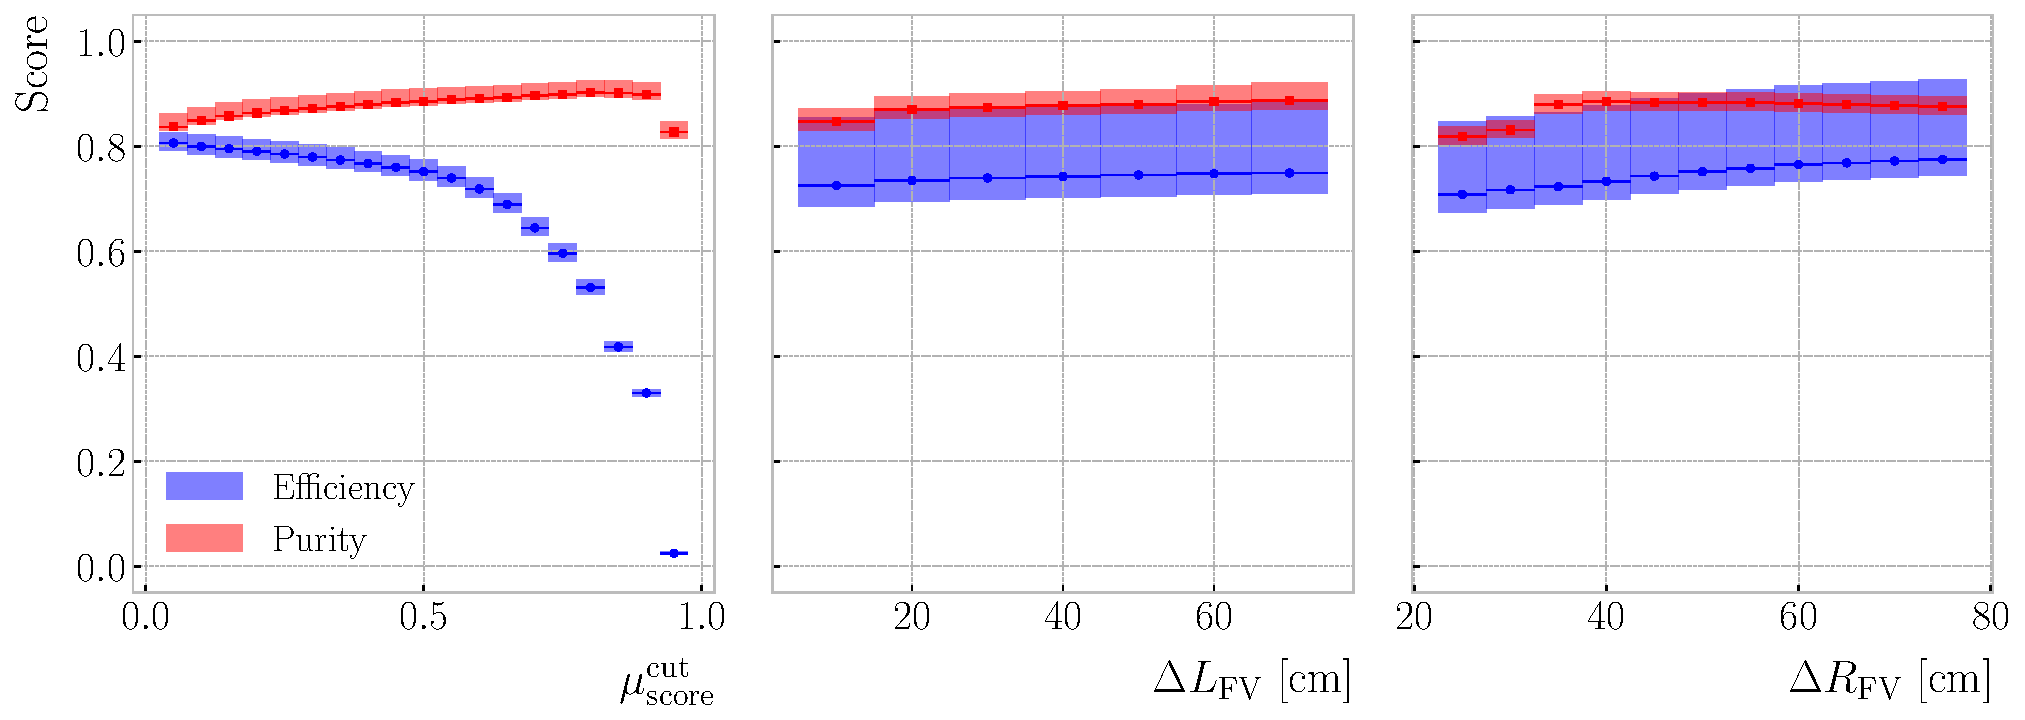
\includegraphics[width=.99\linewidth]{Images/GAr_selection/efficiency_and_purity_error_boxes.pdf}
    \caption[Efficiency and purity for the $\nu_{\mu}$ CC selection as a function of the different cuts.]{Efficiency (blue) and purity (red) for the $\nu_{\mu}$ CC selection as a function of the muon score cut (left panel), FV half-length cut (middle panel), and radial cut (right panel). The height of the boxes represents the IQR of the conditional distributions, whereas the horizontal line corresponds to the median.}
    \label{fig:numuCC_metrics_opt}
\end{figure}

\begin{figure}[t]
    \centering
    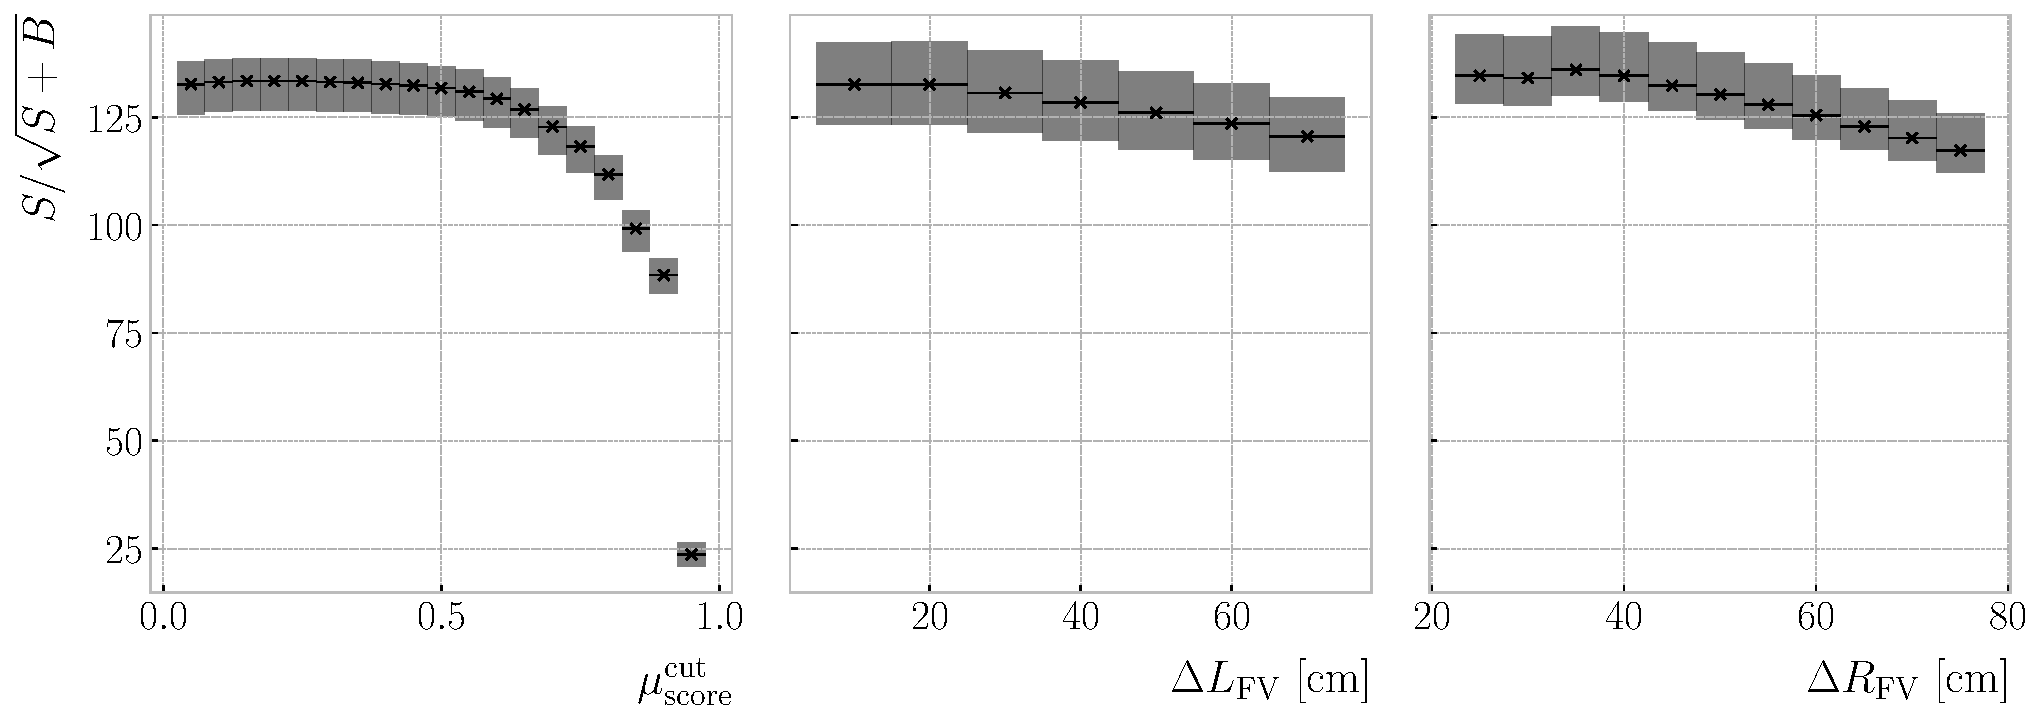
\includegraphics[width=.99\linewidth]{Images/GAr_selection/significance_error_boxes.pdf}
    \caption[Significance for the $\nu_{\mu}$ CC selection as a function of the different cuts.]{Significance for the $\nu_{\mu}$ CC selection as a function of the muon score cut (left panel), FV half-length cut (middle panel), and radial cut (right panel). The height of the boxes represents the IQR of the conditional distributions, whereas the horizontal line corresponds to the median.}
    \label{fig:numuCC_significance_opt}
\end{figure}

Figure \ref{fig:numuCC_metrics_opt} shows the change in efficiency (blue) and purity (red) of the $\nu_{\mu}$ CC selection as a function of the different cuts. From left to right, I vary $\mu_{\mathrm{score}}^{\mathrm{cut}}$, $\Delta L_{\mathrm{FV}}$, and $\Delta R_{\mathrm{FV}}$. For each value of the cuts, I compute the median and IQR (represented by the horizontal lines and the heights of the boxes, respectively) of the corresponding conditional distributions of efficiency and purity. This representation is useful to get an idea of the general trend the scores follow with the cuts, as well as the spread. It is clear that the muon score cut has the biggest impact on the efficiency, which ranges between $0.05$ to $0.80$, whereas the purity remains stable with values around $0.85$.

\begin{comment}
    \begin{figure}[t]
    \centering
    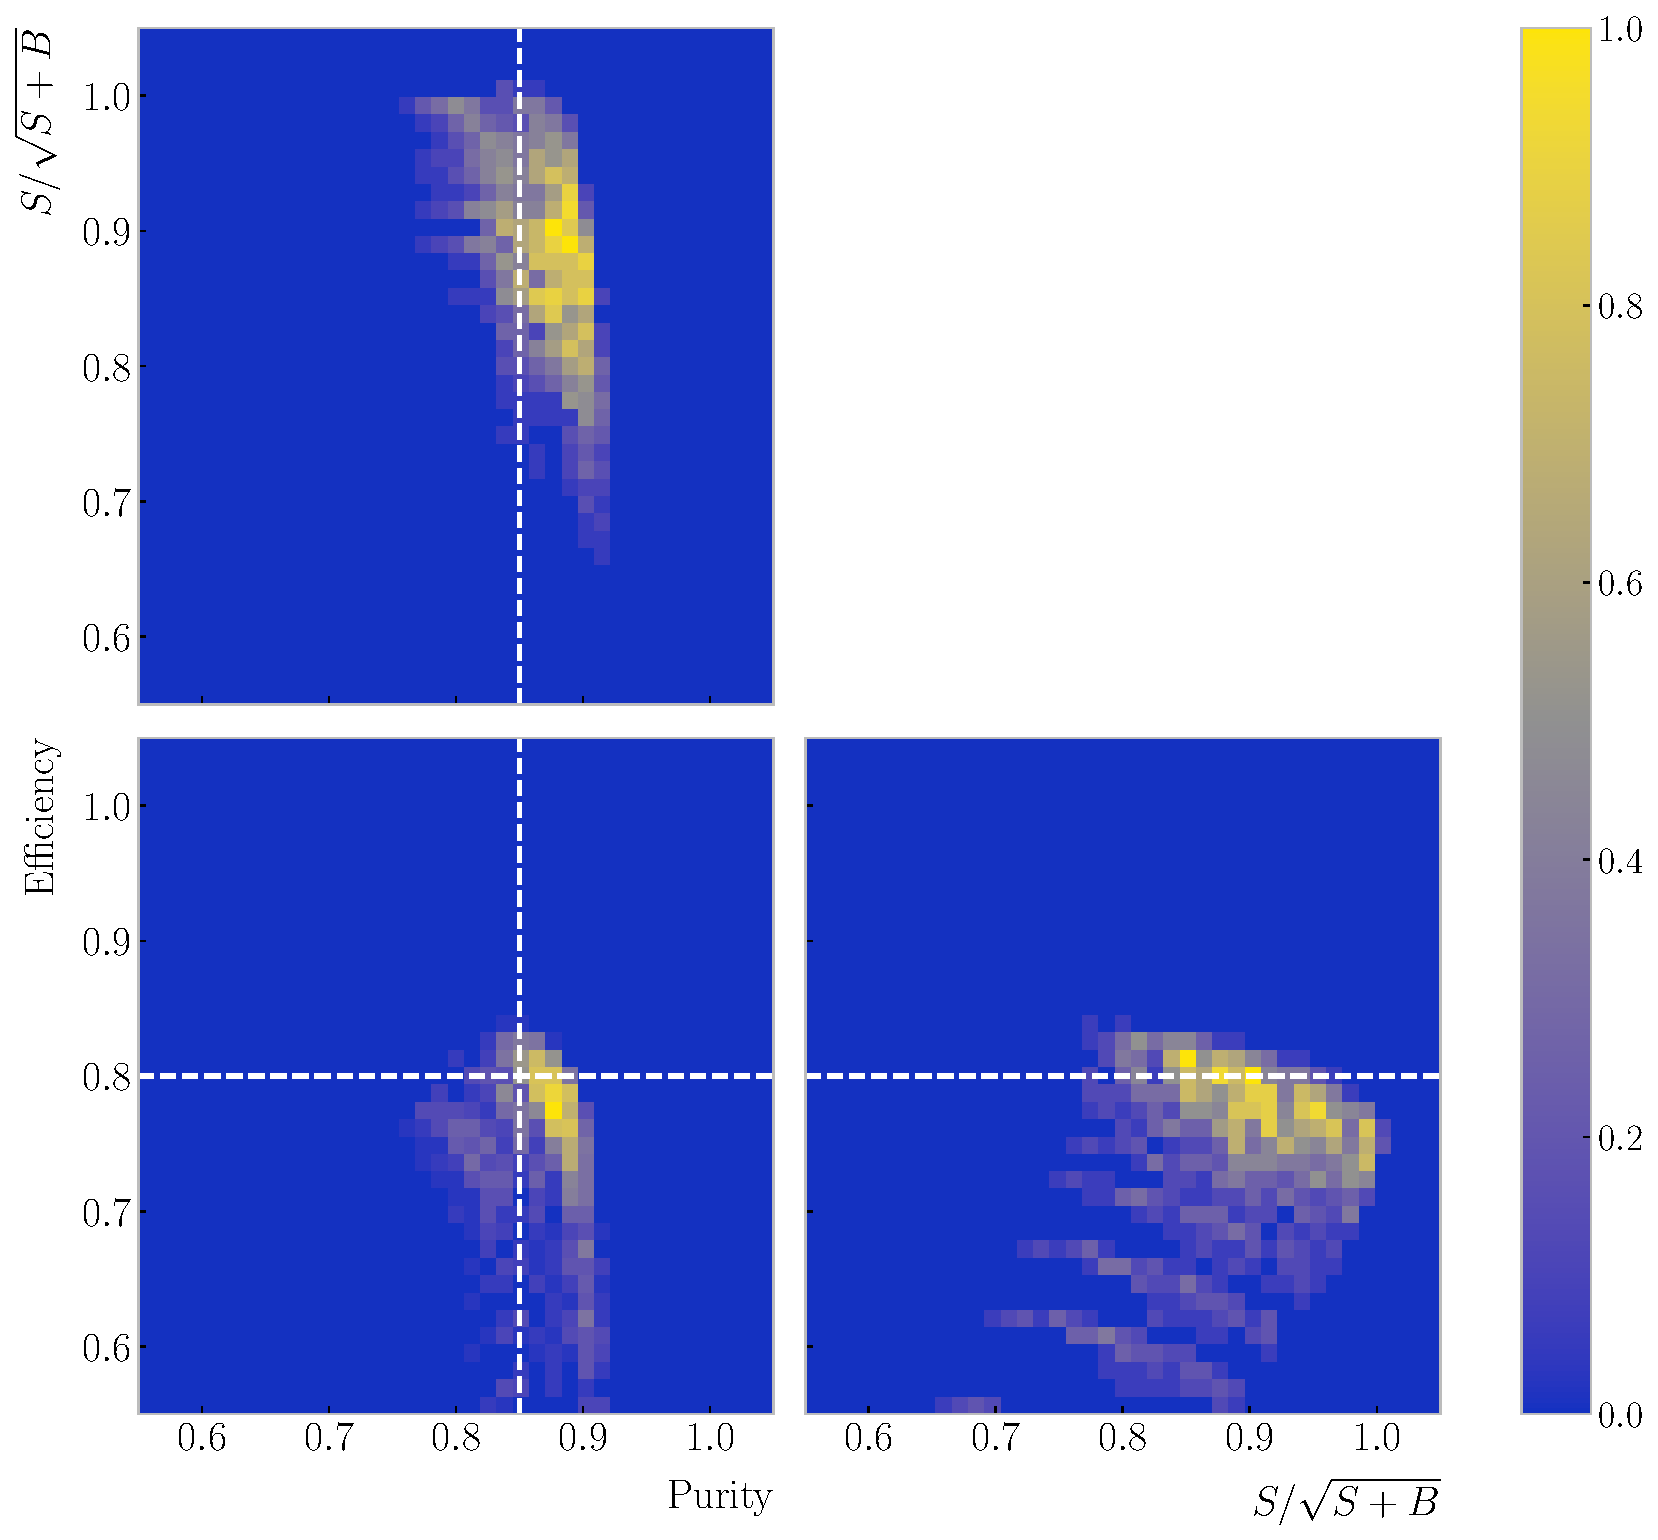
\includegraphics[width=.95\linewidth]{Images/GAr_selection/numuCC_metric_heatmap.pdf}
    \caption{Normalised 2D distributions of efficiency, purity and significance for the $\nu_{\mu}$ CC selection. The $S/\sqrt{S+B}$ is normalised to the highest value achieved. The vertical dashed line indicates a purity value of $0.85$, whereas the horizontal one corresponds to an efficiency of $0.80$.}
    \label{fig:numuCC_metric_heat}
\end{figure}
\end{comment}

A similar depiction of the significance can be found in Fig. \ref{fig:numuCC_significance_opt}. In this case, one can see that the $S/\sqrt{S+B}$ decreases as the cuts grow tighter. However, there are hints of local maxima at intermediate values.

\begin{comment}
    Selecting the cut configuration with the highest significance, $147 \pm 11$ for the parameter values explored here, results in an efficiency and purity of $0.754 \pm 0.006$ and $0.833 \pm 0.007$, respectively. Figure \ref{fig:numuCC_metric_heat} shows the 2D distributions resulting when combining pairs of efficiency, purity and significance, obtained for the cut configurations explored. The significance is normalised to the highest value obtained in the parameter scan. Looking at this, it is clear that a selection with highest efficiency and purity can be achieved, maintaining a similar significance level.
\end{comment}

Selecting the cut configuration with the highest significance, $147 \pm 11$ for the parameter values explored here, results in an efficiency and purity of $0.754 \pm 0.006$ and $0.833 \pm 0.007$, respectively. However, there are other selections which allow to achieve higher efficiencies and purities, maintaining similar significance values.

\begin{figure}[t]
	\centering
	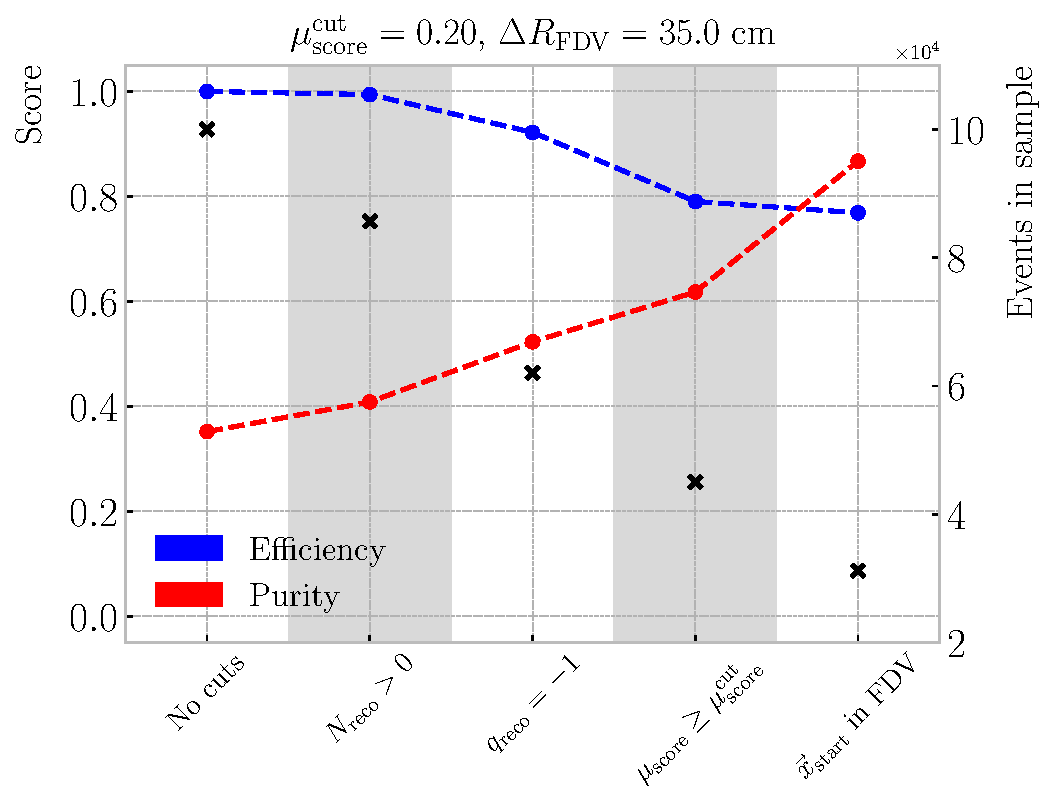
\includegraphics[width=.90\linewidth]{Images/GAr_selection/numu_cc_selection_steps.pdf}
	\caption[Cumulative efficiency and purity for the $\nu_{\mu}$ CC selection.]{Cumulative efficiency (blue) and purity (red) of the $\nu_{\mu}$ CC selection. The secondary axis indicates the number of events in the sample after each cut (black crosses).}
	\label{fig:numuCC_selection_steps}
\end{figure}

\begin{table}[h!]
	\caption[Step-by-step $\nu_{\mu}$ CC selection cuts and cumulative passing rates.]{Step-by-step $\nu_{\mu}$ CC selection cuts and cumulative passing rates. Relative passing rates are indicated in parentheses.}
	\begin{center}
		\begin{small}
			\begin{tabular}{c|ccc}
                Cut \# & Selection cut                       & Events & Passing rates          \\[2mm] \hline
                \rule{0pt}{1.1\normalbaselineskip}0      & Total number of events (No cuts)    & 100000 & $100.00\% ~(100.00\%)$ \\[2mm]
                1      & At least one reconstructed particle                              & 85680  & $85.68 \% ~(85.68 \%)$ \\[2mm]
                2      & Negatively charged particles only                                & 62054  & $62.05\% ~(72.43\%)$   \\[2mm]
                3      & $\mu_{\mathrm{score}} \geq \mu_{\mathrm{score}}^{\mathrm{cut}}$  & 46585  & $46.59\% ~(75.07\%)$   \\[2mm]
                4      & Candidate $\vec{x}_{\mathrm{start}}$ in FV                       & 31834  & $31.83\% ~(68.34\%)$  
                \end{tabular}
		\end{small}
	\end{center}
	\label{tab:numuCC_selection}
\end{table}

Therefore, to get a more refined selection, I first select the configurations with a purity and an efficiency higher than $0.85$ and $0.80$, respectively. After that, I select the tuple of cuts yielding the highest significance. The resulting value for the muon score cut is $\mu_{\mathrm{score}}^{\mathrm{cut}} = 0.10$, and the FV is given by $\Delta L_{\mathrm{FV}} = 30.0~\mathrm{cm}$ and $\Delta R_{\mathrm{FV}} = 50.0~\mathrm{cm}$. With these, one obtains a total efficiency of $0.800 \pm 0.007$ and purity of $0.851 \pm 0.008$, with a significance of $138 \pm 11$. Hereafter, I use this optimised selection cuts, unless specified otherwise.

\begin{figure}[t]
	\centering
	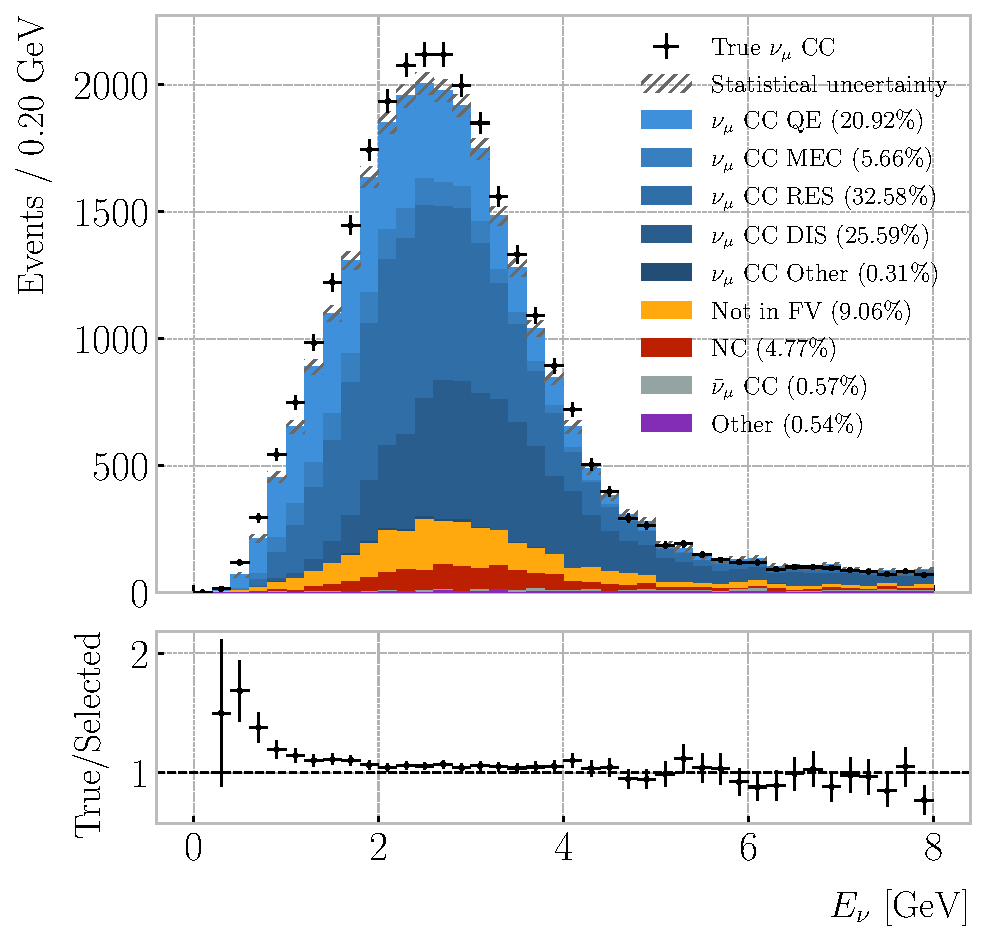
\includegraphics[width=.80\linewidth]{Images/GAr_selection/numuCC_selection_true_energy.pdf}
	\caption[True neutrino energy spectra for the $\nu_{\mu}$ CC selection.]{True neutrino energy spectra for the $\nu_{\mu}$ CC selection. The selected events correspond to the coloured stacked histogram, broken down by signal and background subcategories. The statistical uncertainty is drawn in hatched gray. The true distribution is also shown with the black data points. The bottom panel shows the ratio between the number of true and selected $\nu_{\mu}$ CC events per bin.}
	\label{fig:numuCC_selection_true_enu}
\end{figure}

A summary of the selection can be found in Tab. \ref{tab:numuCC_selection}. It shows the number of events in the selected sample after each selection cut, as well as the absolute and relative passing rates. Figure \ref{fig:numuCC_selection_steps} shows the overall efficiencies (blue) and purities (red) after each cut in the event selection is applied. As expected, the efficiency drops while the purity increases with the successive cuts.

Notice how, out of the cuts prior to the FV constraint, the sign selection produces the highest increase in purity. This is one of the advantages of having a magnetised TPC, and can also be used for a $\bar{\nu}_{\mu}$ CC selection when running in RHC mode.

\begin{figure}[t]
	\centering
	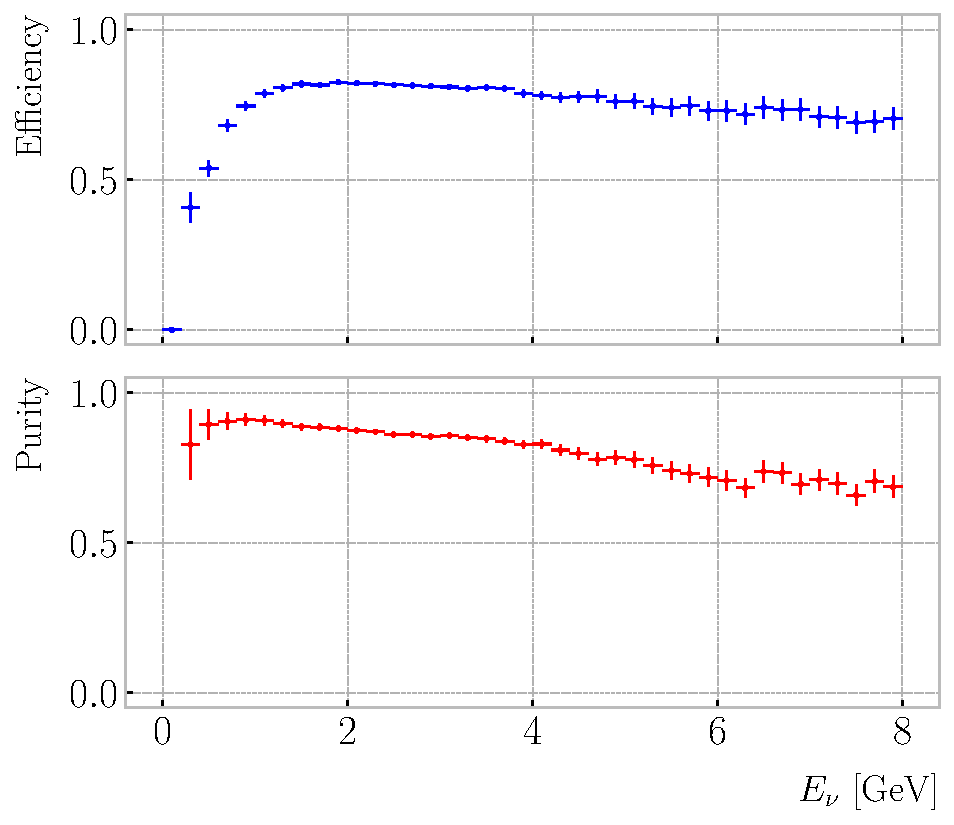
\includegraphics[width=.70\linewidth]{Images/GAr_selection/numuCC_selection_true_energy_performance.pdf}
	\caption[Efficiency and purity for the $\nu_{\mu}$ CC selection as a function of the true neutrino energy.]{Efficiency (top panel) and purity (bottom panel) for the $\nu_{\mu}$ CC selection as a function of the true neutrino energy.}
	\label{fig:numuCC_selection_true_enu_performance}
\end{figure}

\subsection{Selection performance}

Using the stored spectra discussed above, the true neutrino energy distribution for the selected events can be recovered computing $\mathrm{TP}+\mathrm{FP}$. Similarly, the combination $\mathrm{TP}+\mathrm{FN}$ gives the true spectrum. Figure \ref{fig:numuCC_selection_true_enu} shows the true (black data points) and selected (coloured stacked histogram) $E_{\nu}$ distributions for the optimised $\nu_{\mu}$ CC selection. The colours in the selected spectrum indicate the different signal categories and backgrounds, with the overall statistical uncertainty represented by the gray hatched mess. The ratio between the true and selected events is also shown (bottom panel). One can see that it sits around $1$ for most of the energy range. However, for energies $\leq 1~\mathrm{GeV}$ there is a significant deficit of selected events.

\begin{figure}[t]
	\centering
	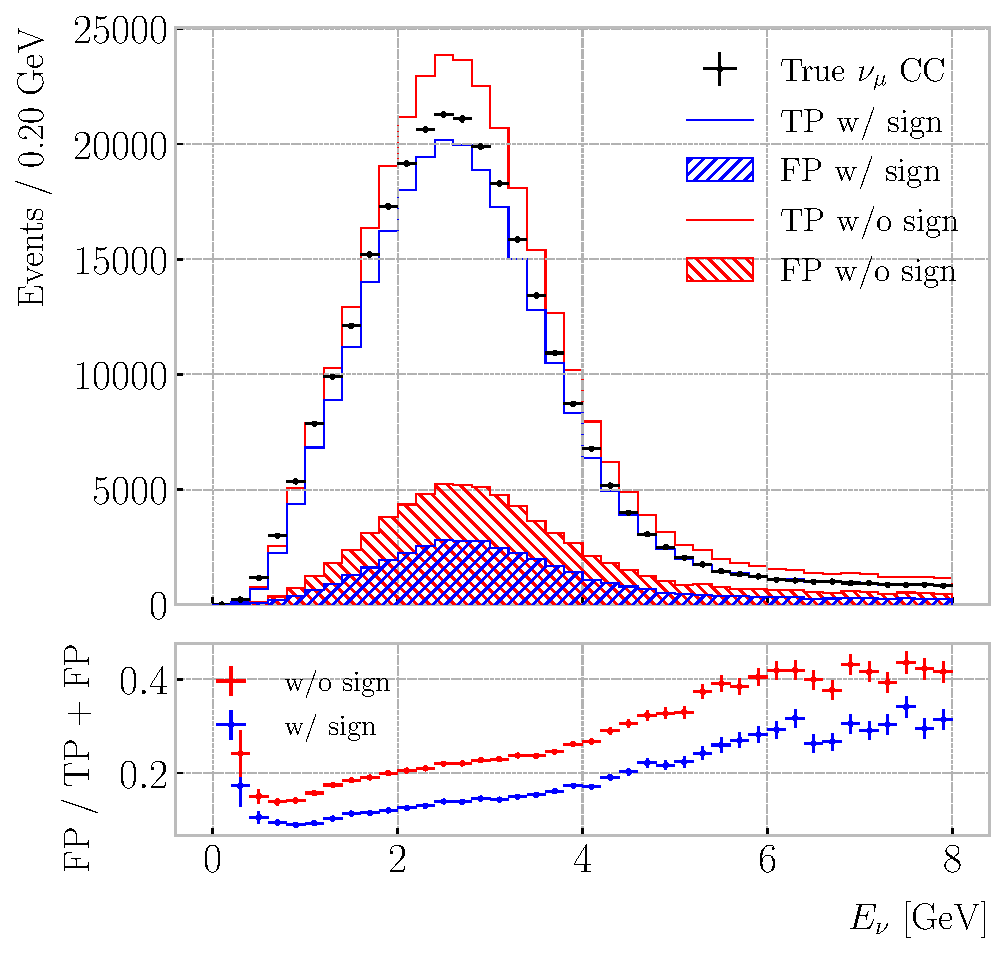
\includegraphics[width=.80\linewidth]{Images/GAr_selection/numuCC_selection_true_energy_sign_comp.pdf}
	\caption{True neutrino energy spectra for the $\nu_{\mu}$ CC selection with (blue) and without (red) sign selection. The selected events are broken down by true positives (signal) and false positives (background). The true distribution is also shown (black data points). The bottom panel shows the ratios between the number of false positives and total selected events per bin.}
	\label{fig:numuCC_sign_selection}
\end{figure}

These spectra also allow to compute the efficiency and purity of the selection as a function of the true neutrino energy, as shown in Fig. \ref{fig:numuCC_selection_true_enu_performance}. As it could be expected from the previous ratio plot, the efficiency is low at low neutrino energies. Nonetheless, it raises quickly with the energy, until it stabilises around a value of $0.80$. Looking at the purity, one may notice that, although it starts at around $0.90$, there is a significant decrease towards the high end of the spectrum.

A variation of the $\nu_{\mu}$ CC selection one can try is to apply it without the reconstructed charge cut. Figure \ref{fig:numuCC_sign_selection} (top panel) shows the $E_{\nu}$ distributions corresponding to the selection with (blue stacked histogram) and without (red stacked histogram) the sign selection. In the former case, the out of FV contamination amounts to $9.06\%$ of the total, while the NC contamination results $4.77\%$ and the wrong-sign contamination $0.57\%$. For the latter, these backgrounds account for the $10.01\%$, $10.82\%$, and $2.18\%$ of the selected events, respectively. As expected, removing the positive particles does not change the FV-related effects noticeably. However, the sign selection proves its worth in the rejection of $\bar{\nu}_{\mu}$ CC events, which drop almost by one order of magnitude. Additionally, the charge selection cuts the NC events in half, as it reduces the chances of misidentifying a positively charged hadron for a muon.

\begin{figure}[t]
	\centering
	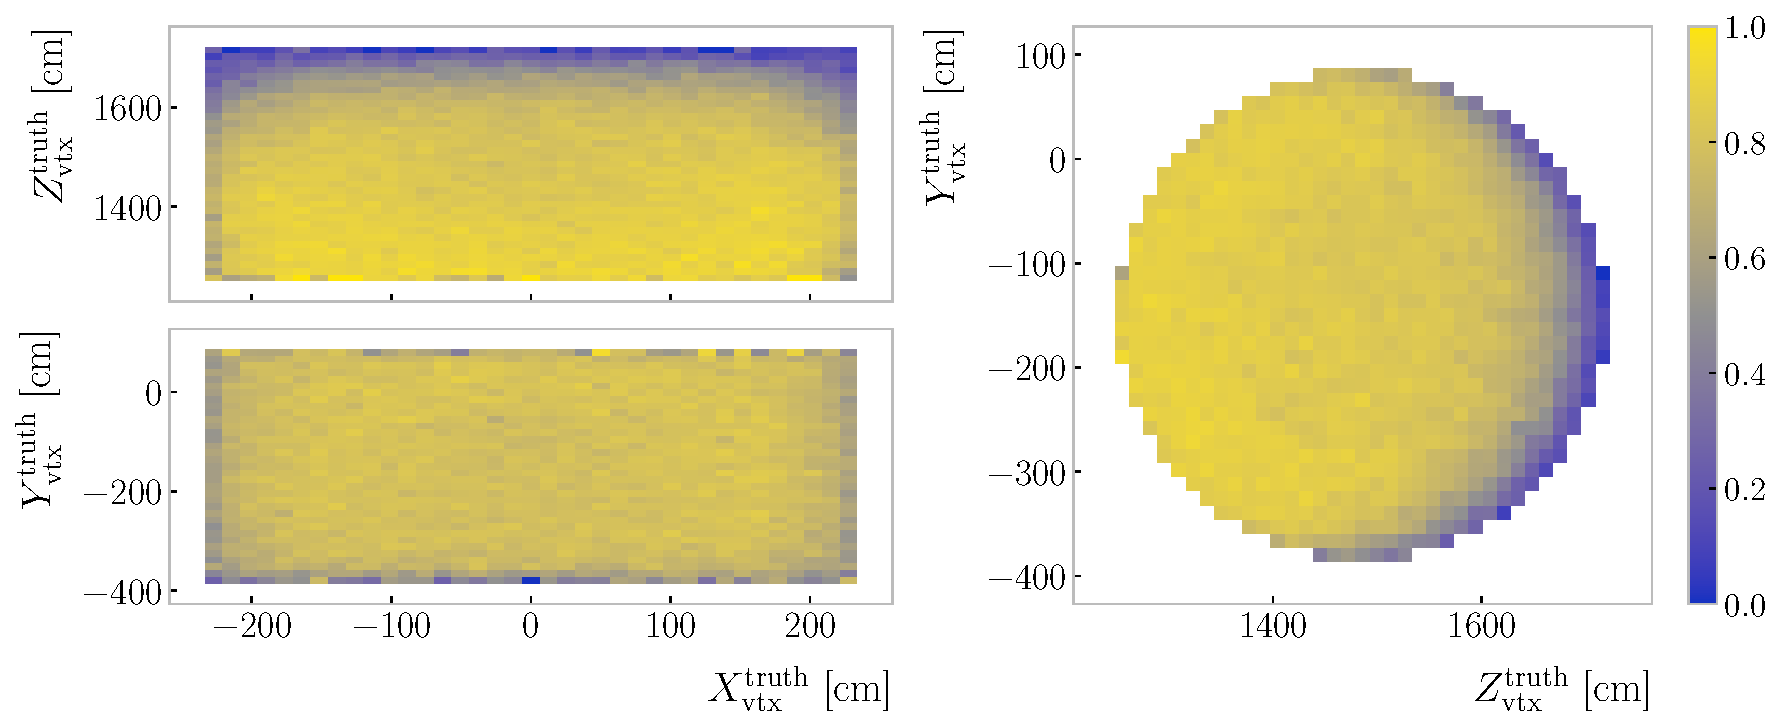
\includegraphics[width=.99\linewidth]{Images/GAr_selection/numuCC_selection_true_vertex_performance.pdf}
	\caption{Efficiency 2D distributions for the $\nu_{\mu}$ CC selection given the true position of the interaction vertex.}
	\label{fig:numuCC_vertex_efficiency}
\end{figure}

As an additional check, I explored how the performance of the $\nu_{\mu}$ CC selection depends on the position of the neutrino interaction within the HPgTPC. Maps of the selection efficiency for the $X,Z$ (top left panel), $X,Y$ (bottom left panel), and $Z,Y$ (right panel) true vertex position pairs are given in Fig. \ref{fig:numuCC_vertex_efficiency}. It can be seen that the efficiency remains stable along the drift direction, only slightly degrading close to the edges of the FV. Regarding the radial direction, it is clear that an important number of events with high $Z^{\mathrm{truth}}_{\mathrm{vtx}}$ are not being selected. Intuitively, the muons arising from these interactions will leave short tracks. As their directions are typically aligned with the beam direction, they enter the ECal shortly after production. This is likely to affect the tracking, and therefore their identification. As a result, the regions with the lowest efficiency are the downstream corners of the HPgTPC, i.e. the areas with high $|X^{\mathrm{truth}}_{\mathrm{vtx}}|$ and $Z^{\mathrm{truth}}_{\mathrm{vtx}}$.

\begin{comment}
\begin{figure}[t]
	\begin{subfigure}{0.5\textwidth}
		\centering
		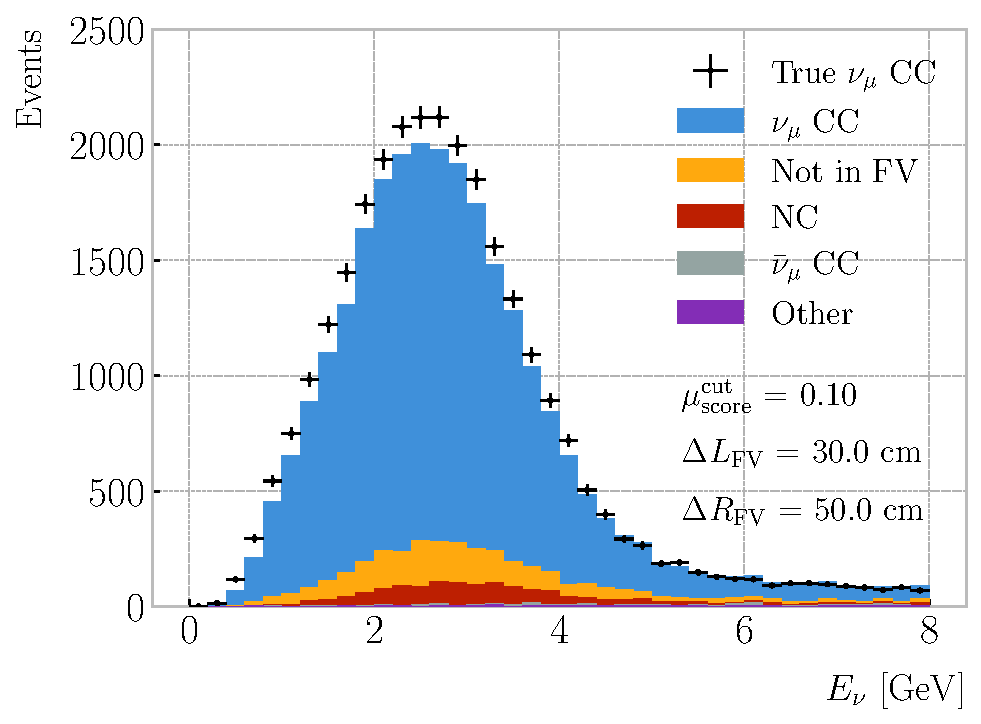
\includegraphics[width=.99\linewidth]{Images/GAr_selection/nu_energy_with_breakdown.pdf}
	\end{subfigure}
	\begin{subfigure}{0.5\textwidth}
		\centering
		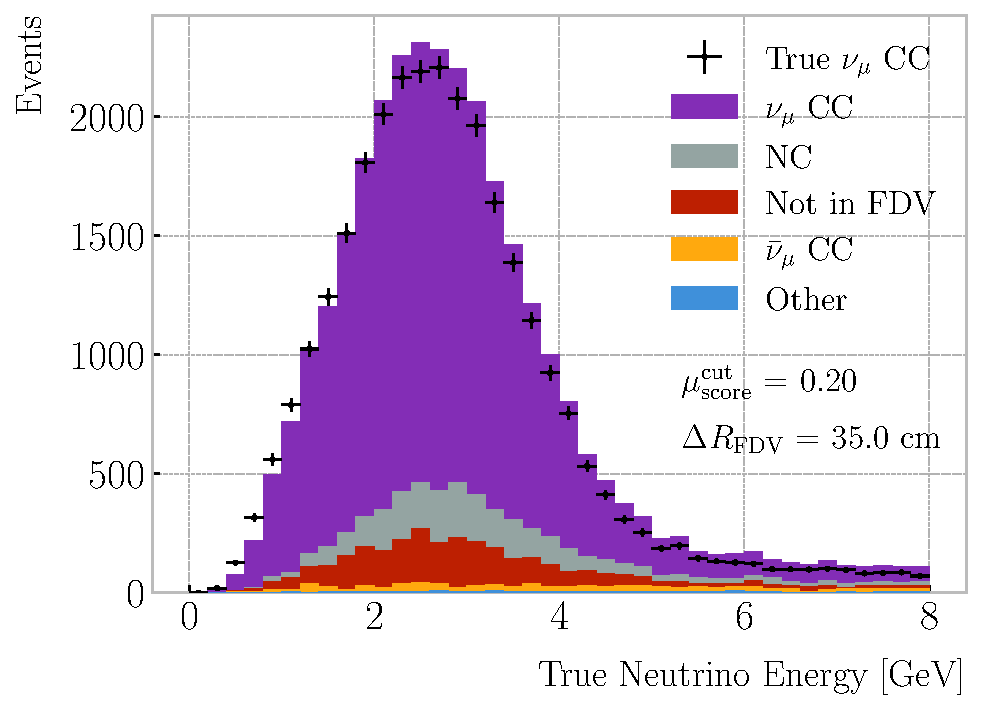
\includegraphics[width=.99\linewidth]{Images/GAr_selection/nu_energy_with_breakdown_no_sign.pdf}
	\end{subfigure}
	\caption[True neutrino energy spectra for the $\nu_{\mu}$ CC selection with and without sign selection.]{True neutrino energy spectra for the $\nu_{\mu}$ CC selection with (left panel) and without (right panel) sign selection. The selected events are broken down by signal or background category. The true distribution is also shown (black data points).}
	\label{fig:numuCC_sign_selection}
\end{figure}
\end{comment}

\begin{figure}[t]
    \centering
    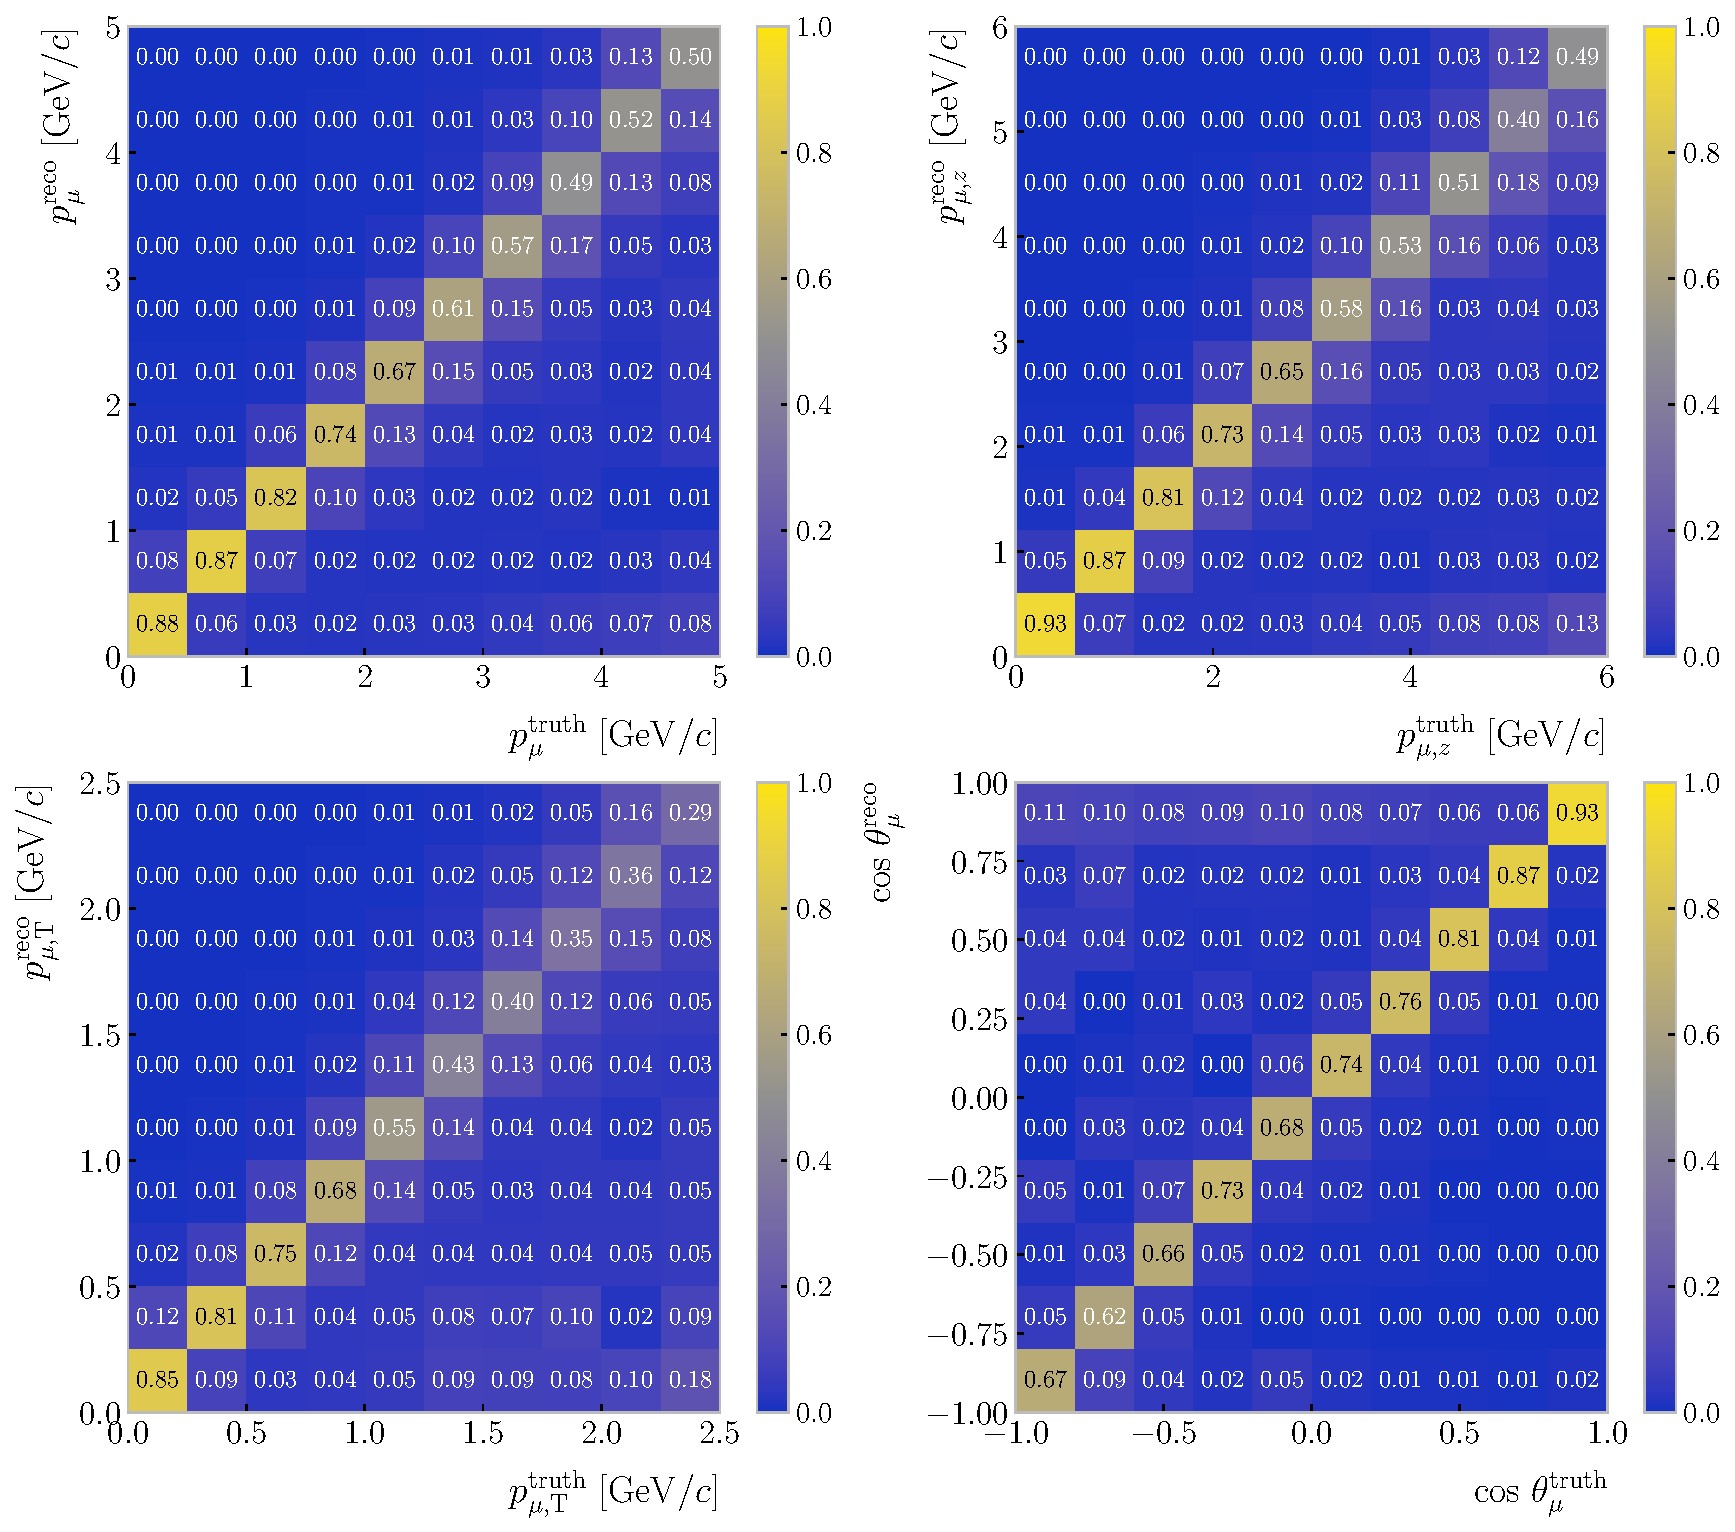
\includegraphics[width=.99\linewidth]{Images/GAr_selection/numuCC_muon_kinematic_comp.pdf}
    \caption[Distributions for the reconstructed versus truth primary muon momentum, longitudinal momentum, transverse momentum, and angle.]{Distributions for the reconstructed versus truth generated primary muon momentum (top left panel), longitudinal momentum (top right panel), transverse momentum (bottom left panel), and beam angle (bottom right panel). The reconstructed values correspond to the selected primary muon candidate, whereas the truth values come from the true primary muon in the event.}
    \label{fig:numuCC_muon_kinematic_comp}
\end{figure}

\subsection{Primary muon kinematics}

This $\nu_{\mu}$ CC selection relies on the identification of the a primary muon, meaning that for each selected event a particle is picked out as the muon candidate. It is because of this that one can study the kinematics of these selected primary muons.

Figure \ref{fig:numuCC_muon_kinematic_comp} shows a comparison between some of the reconstructed and truth primary muon kinematic variables. From top to bottom, left to right, we have muon momentum, longitudinal momentum, transverse momentum, and beam angle. The histograms are column-normalised, and so the diagonal entries give an idea of the resolution for the different variables. The match between truth and reconstructed values can only be done for the selected true $\nu_{\mu}$ CC events, as the others do not have a primary muon. However, for this comparison I do not require the events to start inside the FV.

\begin{figure}[t]
	\centering
	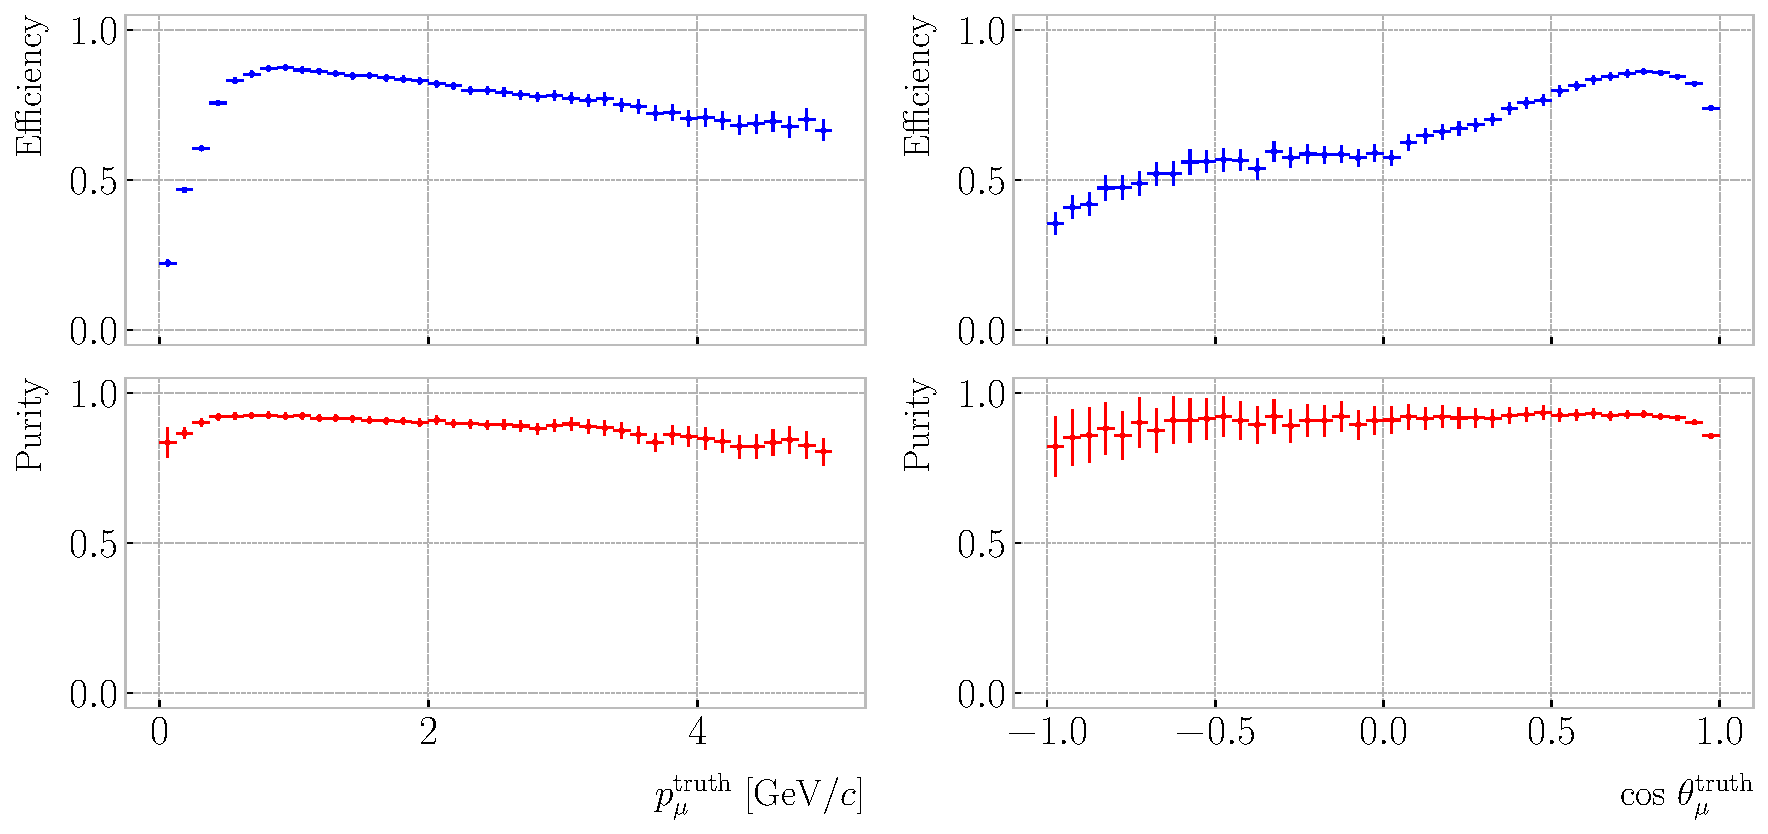
\includegraphics[width=.99\linewidth]{Images/GAr_selection/numuCC_selection_true_kinematics_performance.pdf}
	\caption[Efficiency and purity of the $\nu_{\mu}$ CC selection as a function of the primary muon true momentum and beam angle.]{Efficiency (blue) and purity (red) of the $\nu_{\mu}$ CC selection as a function of the primary muon true momentum (left panel) and beam angle (right panel).}
	\label{fig:numuCC_muon_kinematics}
\end{figure}

Notice that, for the reconstructed values, the variables do not necessarily come from a reconstructed particle that matches the true primary muon. In other words, sometimes, even though the event was correctly identified, the primary muon may have been confused with another particle. That means that in these distributions include both reconstruction and selection deficiencies.

\begin{figure}[p!]
    \centering
    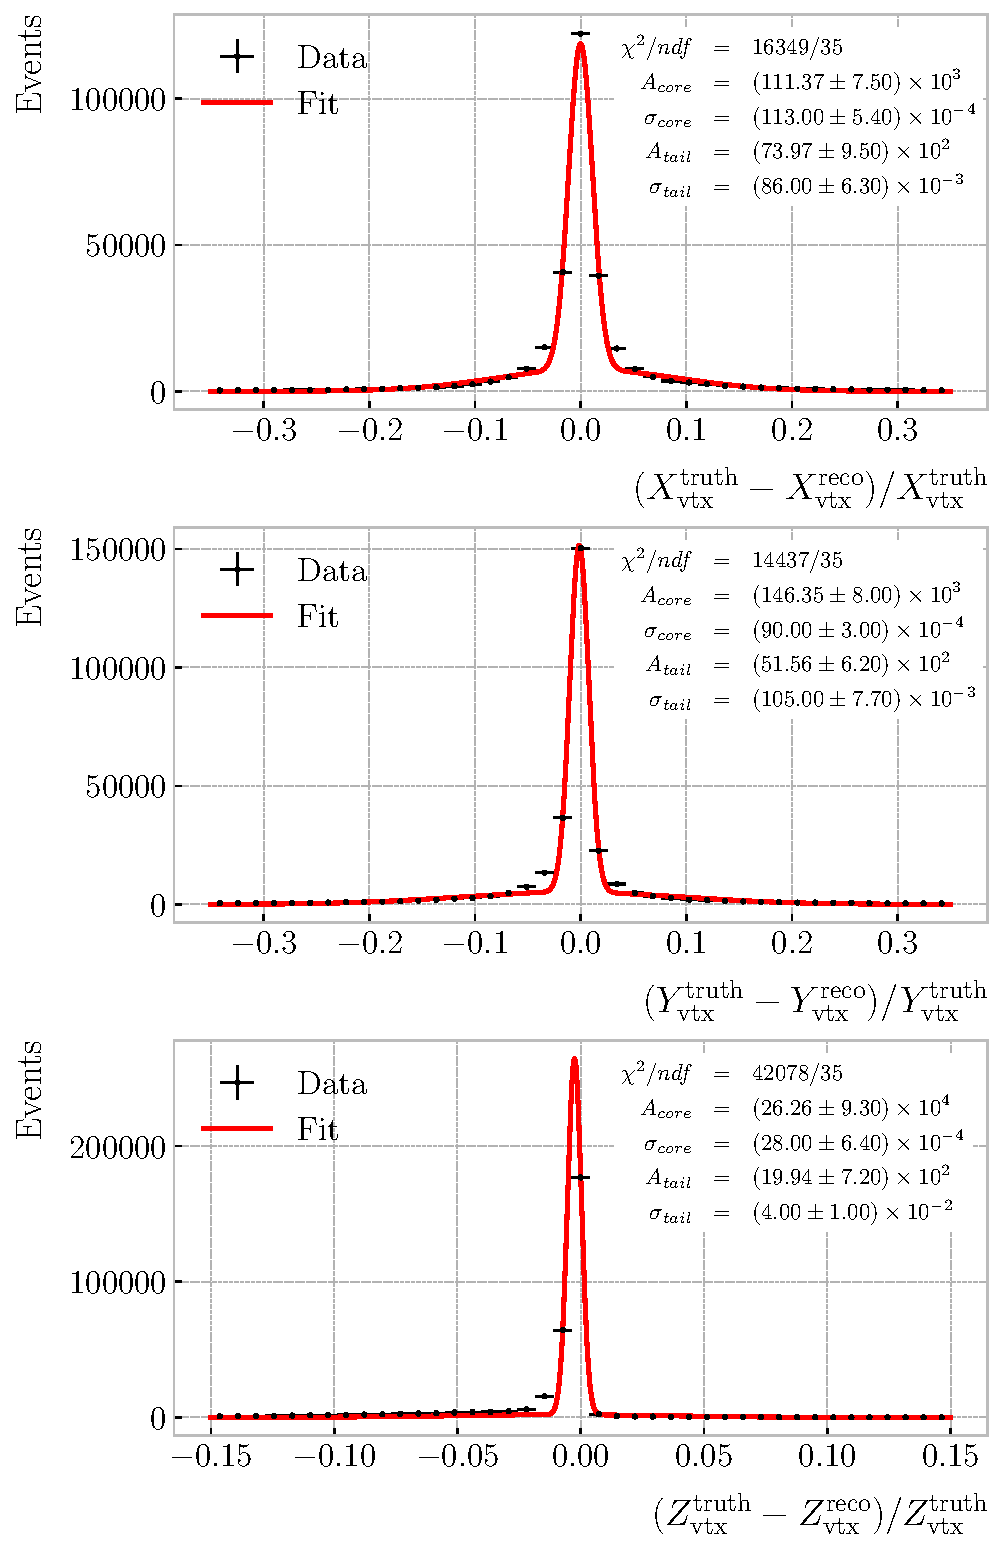
\includegraphics[width=.80\linewidth]{Images/GAr_selection/numuCC_muon_vtx_residuals.pdf}
    \caption[Fractional residual distributions for the position of the primary vertex in the $\nu_{\mu}$ CC selection.]{Fractional residual distributions for the position of the primary vertex in the $\nu_{\mu}$ CC selection. The best fits to a double Gaussian function are also shown (red lines).}
    \label{fig:numuCC_vertex_residuals}
\end{figure}

I also studied the performance of the $\nu_{\mu}$ CC selection as a function of the kinematic variables of the primary muon. As before, these metrics are only possible to compute for true $\nu_{\mu}$ CC events. The efficiency (top panels) and purity (bottom panels) as a function of the truth muon momentum (left) and beam angle (right) are shown in Fig. \ref{fig:numuCC_muon_kinematics}. One can see that there are some similarities in the behaviour of both metrics between the true neutrino energy and the muon momentum cases. This is to be expected, as these two variables are highly correlated. For the efficiency, there is a rapid increase at low momentum values until it peaks at around $1~\mathrm{GeV}/c$, after which it starts decreasing slowly. The purity remains relatively constant, with a slight drop towards high $p_{\mu}^{\mathrm{truth}}$ values. In the case of the muon angle, the decrease in efficiency at high $\theta_{\mu}^{\mathrm{truth}}$ is more noticeable. However, note that the number of events with backward-going muons is much smaller than those aimed towards the forward direction, as can be seen from the size of the vertical error bars. There is also a decrease in the purity with the beam angle, but this effect is much smaller.

A byproduct of selecting the primary lepton in the interaction is the position of the reconstructed neutrino vertex candidate. Checking how the position of the selected reconstructed primary vertex and the true vertex position compare is needed to understand the validity of our method. Figure \ref{fig:numuCC_vertex_residuals} shows the distributions of fractional residuals between the truth and reconstructed vertex positions in the $X$ (top panel), $Y$ (middle panel), and $Z$ (bottom panel) directions. Performing a double Gaussian fit to the distributions (red lines), I estimate the reconstructed vertex resolution achieved with this method to be $1.62 \pm 0.08 \%$, $1.23 \pm 0.05 \%$, and $0.32 \pm 0.05 \%$ for the $X$, $Y$, and $Z$ directions, respectively. As expected, the resolution along the drift direction is slightly worse. However, the significant difference in resolution between the two transverse directions is worth noting. Not only the resolution is better for the $Z$ direction, but the layout of the residual distribution is highly asymmetrical. This may be related to the variability in the selection efficiency along that direction.

\begin{comment}
\begin{figure}[t]
    \centering
    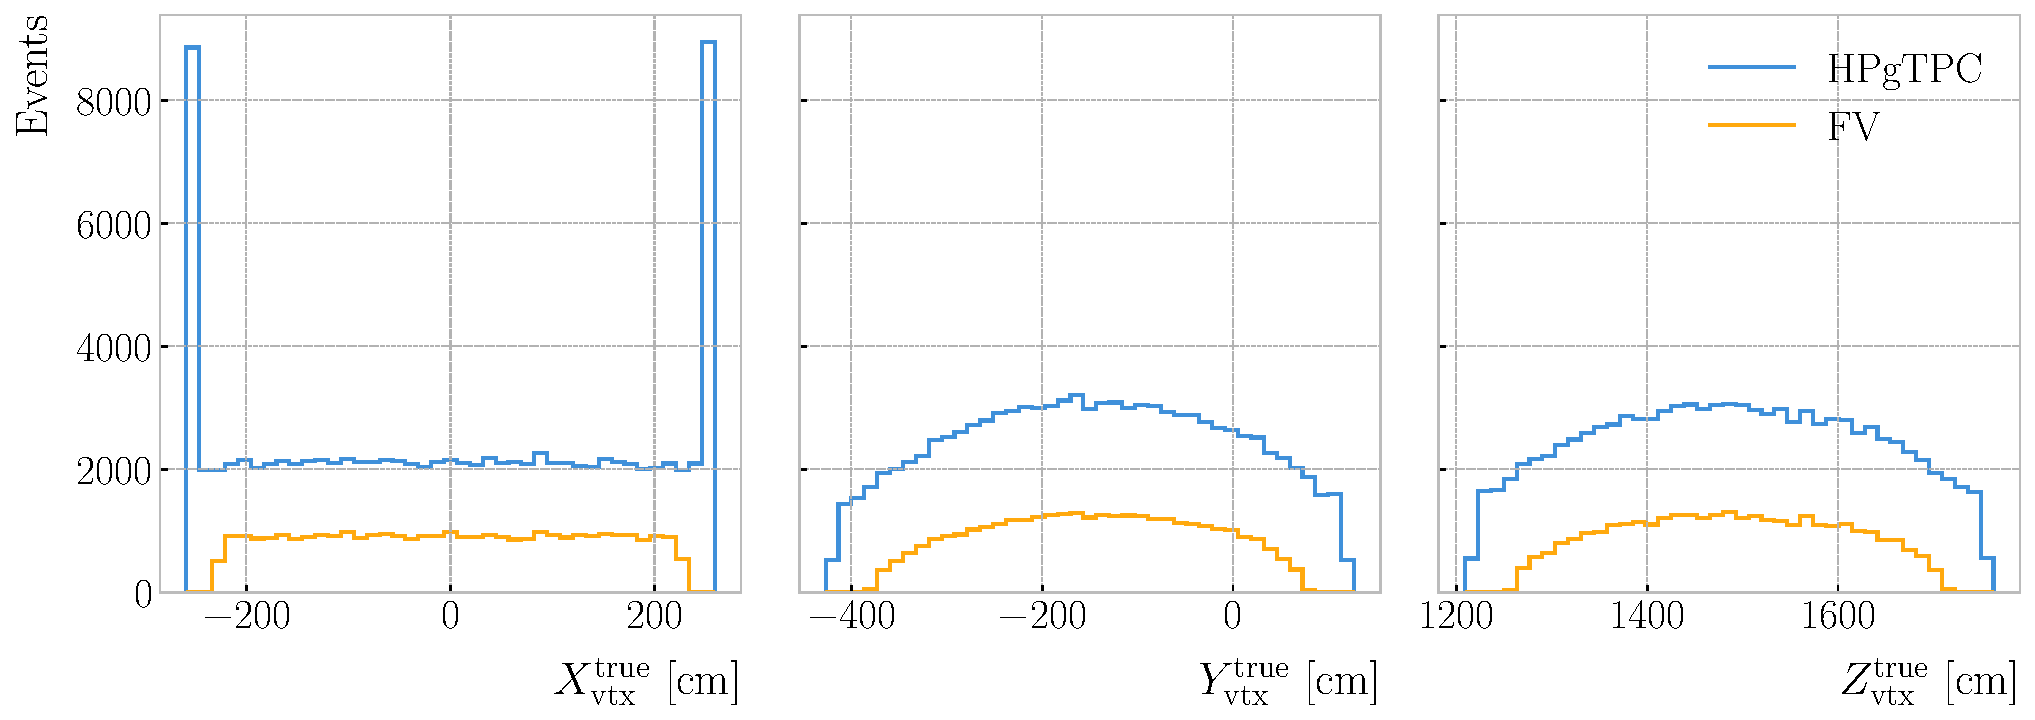
\includegraphics[width=.99\linewidth]{Images/GAr_selection/numuCC_true_vertex_position_fiducial.pdf}
    \caption[Distributions of the true $\nu_{\mu}$ CC vertex positions for the full HPgTPC and the FV.]{Distributions of the true $\nu_{\mu}$ CC vertex positions for the full HPgTPC volume (blue) and the optimised FV (yellow), given by $\Delta L_{\mathrm{FV}} = 30.0 ~ \mathrm{cm}$ and $\Delta R_{\mathrm{FV}} = 50.0 ~ \mathrm{cm}$.}
    \label{fig:numuCC_true_vertex}
\end{figure}
\end{comment}

\section{Charged pion identification}
\label{sec:gar_charged_pions}

Now that I have checked the robustness of the proposed $\nu_{\mu}$ CC selection, it can be used as a starting point for other, more convoluted, selections. One of the priorities of ND-GAr, as mentioned previously, is the identification of pions. With its lower tracking thresholds, ND-GAr is expected to do better regarding $\pi^{\pm}$ identification than the traditional LArTPCs, like ND-LAr. Moreover, it can make use of the different detector subcomponents to tag the charged pions.

\begin{figure}[t]
    \centering
    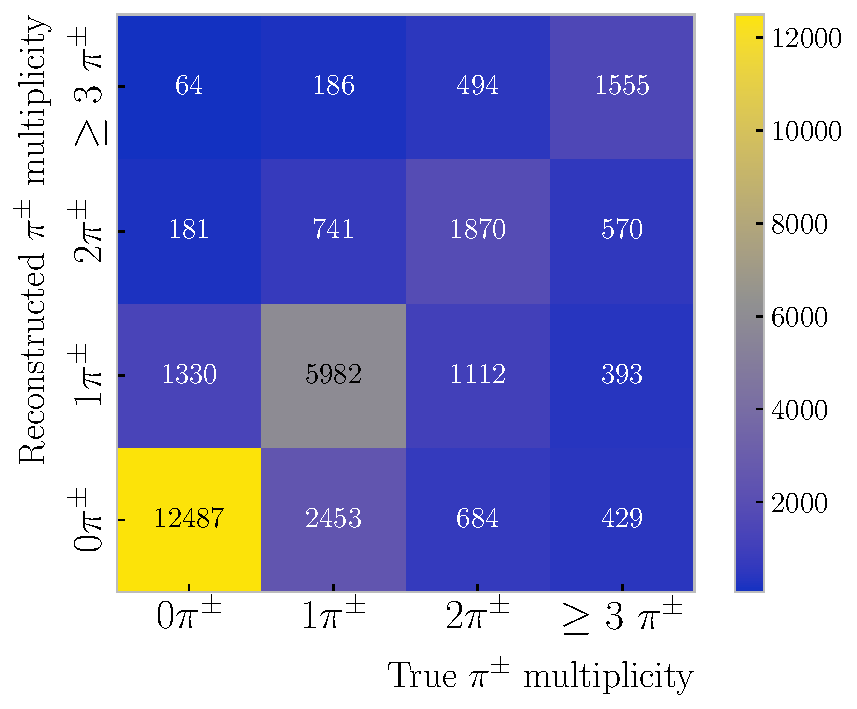
\includegraphics[width=.75\linewidth]{Images/GAr_selection/pion_selection_confusion_matrix.pdf}
    \caption[Distribution of events based on their true and reconstructed $\pi^{\pm}$ multiplicity, for a given selection.]{Distribution of events based on their true and reconstructed $\pi^{\pm}$ multiplicity, for the selection given by $p^{\mathrm{cut}}_{\mathrm{d}E/\mathrm{d}x} = p^{\mathrm{cut}}_{\mathrm{ToF}} = 0.50$, $\Delta^{\pi^{\pm}}_{\mathrm{d}E/\mathrm{d}x} = 0.20$, and $d^{\mathrm{cut}}_{\mu} = 50.0~\mathrm{cm}$.}
    \label{fig:pion_multiplicity_example}
\end{figure}

The $\nu_{\mu}$ CC selection provides a starting point for the pion identification. The first thing one can do is rule out the selected primary muon candidate. Then, by looking at the properties of the rest of the reconstructed particles, one can start the counting of the charged pions.

The two proton scores, the one based on the $\mathrm{d}E/\mathrm{d}x$ in the HPgTPC and the one obtained from the ToF measurement in the ECal, can be used to separate the protons from the sample of charged pions. By providing appropriate cuts for these, a good separation can be achieved.

Another source of information available is the $\mathrm{d}E/\mathrm{d}x$ of the track associated to the reconstructed particle. To select the charged pions, we can require that the measured mean $\mathrm{d}E/\mathrm{d}x$ is compatible with the expectation for a true $\pi^{\pm}$, in other words:
\begin{eqnarray}
    \left<\frac{\mathrm{d}E}{\mathrm{d}x}\right>_{\pi^{\pm}} \left(1 - \Delta_{\mathrm{d}E/\mathrm{d}x}^{\pi^{\pm}}\right) \leq \left<\frac{\mathrm{d}E}{\mathrm{d}x}\right>_{\mathrm{meas.}} < \left<\frac{\mathrm{d}E}{\mathrm{d}x}\right>_{\pi^{\pm}} \left(1 + \Delta_{\mathrm{d}E/\mathrm{d}x}^{\pi^{\pm}}\right),
\end{eqnarray}
where the parameter $\Delta_{\mathrm{d}E/\mathrm{d}x}^{\pi^{\pm}}$ measures the fractional variation one allows around the theoretical expectation. To obtain the expected mean $\mathrm{d}E/\mathrm{d}x$ of a charged pion with a given momentum, I use the ALEPH parametrisation with the parameter values obtained previously in section \ref{subsec:dEdx_parametrisation}.

Also, as we are only interested in the primary pions, and because these are by definition close to the interaction vertex, one can apply an additional distance cut. Using the start position of the muon candidate, we can restrict the starting point of the pions to a certain volume around the vertex.

Combining all these ideas, I propose the following procedure to identify the charged pions in an event:
\begin{enumerate}
    \item Apply $\nu_{\mu}$ CC selection.
    \item Disregard particle selected as primary muon.
    \item Remove particles with momentum below threshold.
    \item Select particles with proton $\mathrm{d}E/\mathrm{d}x$ score below threshold.
    \item Select particles with proton ToF score below threshold.
    \item Select particles with mean $\mathrm{d}E/\mathrm{d}x$ around the expected value for a pion.
    \item Remove particles with a distance between the start of the track and the primary vertex greater than the cut.
\end{enumerate}
The remaining particles after all these cuts are taken to be charged pion candidates.

\begin{figure}[t]
    \centering
    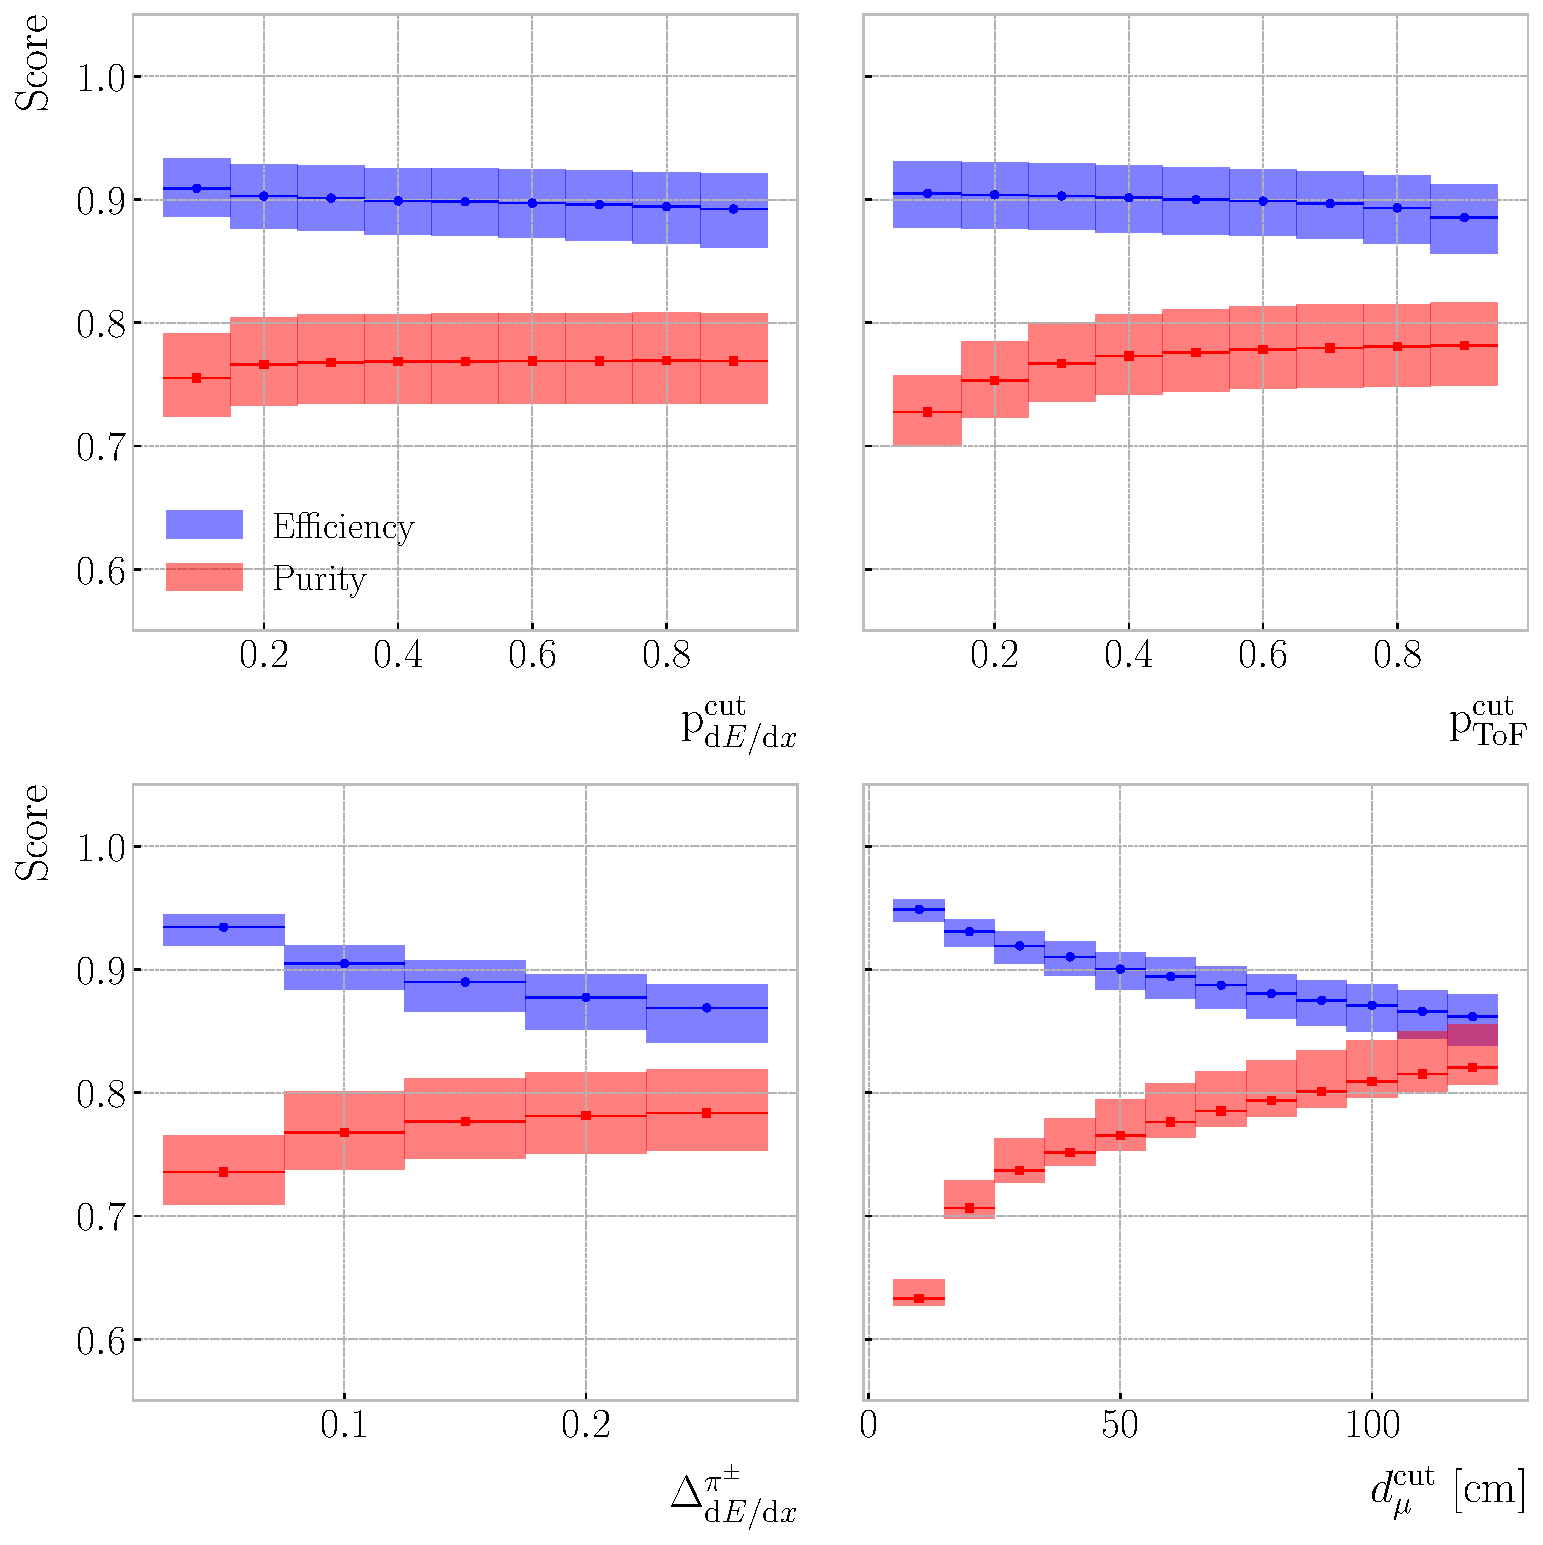
\includegraphics[width=.85\linewidth]{Images/GAr_selection/pion_selection_0_pions_metrics.pdf}
    \caption[Efficiency and purity for the $\nu_{\mu}$ CC $0\pi^{\pm}$ selection as a function of the different cuts.]{Efficiency (blue) and purity (red) for the $\nu_{\mu}$ CC $0\pi^{\pm}$ selection as a function of the proton $\mathrm{d}E/\mathrm{d}x$ score cut (top left panel), proton ToF score cut (top right panel), pion $\mathrm{d}E/\mathrm{d}x$ cut (bottom left panel), and distance to muon cut (bottom right panel). The height of the boxes represents the IQR of the conditional distributions, whereas the line corresponds to the median.}
    \label{fig:pion_selection_0_pions_metrics}
\end{figure}

This counting method depends on four cuts, denoted by $p^{\mathrm{cut}}_{\mathrm{d}E/\mathrm{d}x}$, $p^{\mathrm{cut}}_{\mathrm{ToF}}$, $\Delta^{\pi^{\pm}}_{\mathrm{d}E/\mathrm{d}x}$, and $d^{\mathrm{cut}}_{\mu}$ in order of appearance. The momentum threshold is necessary to compare with the true multiplicity. For values of the kinetic energy lower than $10-20~\mathrm{MeV}$, we do not expect to be able to tag individual pions. Such low energy particles just leave small traces in the TPC which, together with the busy environment of the neutrino interaction vertex, leaves one with no other option but to only account for their energy calorimetrically. As such, the true pion counting also features this momentum threshold.

I performed an optimisation of the charged pion counting by scanning the space of possible cut configurations. For the two proton scores, I let them vary between $0.10$ to $0.90$, in increments of $0.10$. Similarly, the parameter $\Delta^{\pi^{\pm}}_{\mathrm{d}E/\mathrm{d}x}$ takes values in the range $0.05-0.25$, with a step size of $0.05$. Finally, the distance cut changes in $10~\mathrm{cm}$ steps, from $10$ to $120~\mathrm{cm}$.

For each combination of selection cuts, I compare the true charged pion multiplicity given by GENIE with the number of charged pion candidates I count with this method, hereafter referred to as the reconstructed $\pi^{\pm}$ multiplicity. The result of this comparison is a matrix, with columns and rows indicating true and reconstructed charged pion multiplicity, respectively. An example of one of these matrices, obtained for a certain configuration of cuts, can be seen in Fig. \ref{fig:pion_multiplicity_example}. From these multiplicity matrices one can extract performance metrics, like efficiency, purity, and significance.

\begin{figure}[t]
    \centering
    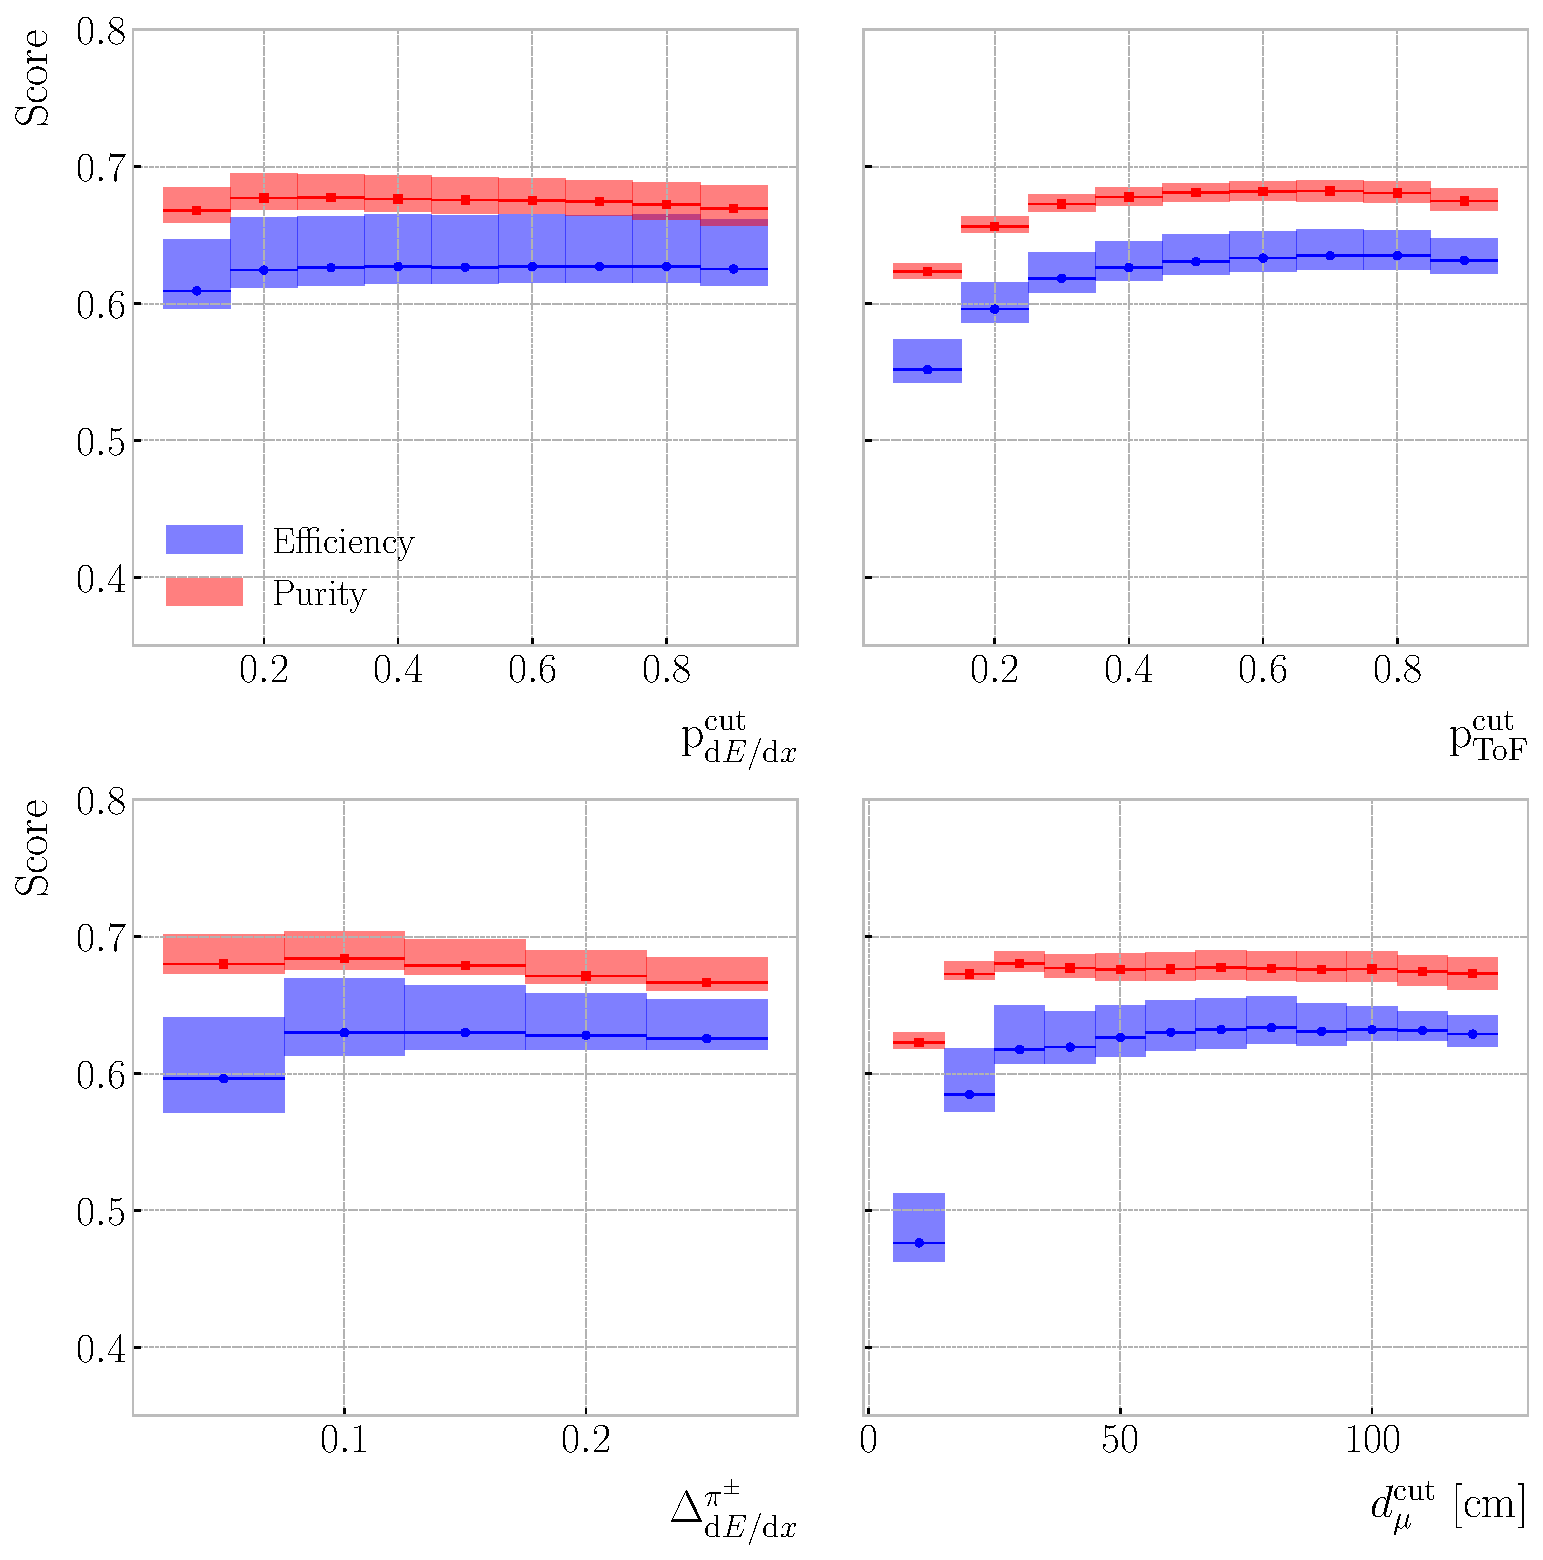
\includegraphics[width=.85\linewidth]{Images/GAr_selection/pion_selection_1_pions_metrics.pdf}
    \caption[Efficiency and purity for the $\nu_{\mu}$ CC $1\pi^{\pm}$ selection as a function of the different cuts.]{Efficiency (blue) and purity (red) for the $\nu_{\mu}$ CC $1\pi^{\pm}$ selection as a function of the proton $\mathrm{d}E/\mathrm{d}x$ score cut (top left panel), proton ToF score cut (top right panel), pion $\mathrm{d}E/\mathrm{d}x$ cut (bottom left panel), and distance to muon cut (bottom right panel). The height of the boxes represents the IQR of the conditional distributions, whereas the line corresponds to the median.}
    \label{fig:pion_selection_1_pions_metrics}
\end{figure}

Given a multiplicity matrix $\mathbf{M}$, the efficiency for the $i$-th multiplicity value can be computed as:
\begin{equation}\label{eq:efficiency_matrix}
    \left.\mathrm{Efficiency}\right|_{i} = \frac{M_{ii}}{\sum_{j} M_{ij}},
\end{equation}
or in other words, dividing the corresponding diagonal entry by the sum of all the entries in the same column. On the other hand, the purity is given by:
\begin{equation}\label{eq:purity_matrix}
    \left.\mathrm{Purity}\right|_{i} = \frac{M_{ii}}{\sum_{j} M_{ji}},
\end{equation}
which is just the ratio between the diagonal entry and the sum of the entries in the corresponding row. Similarly, the significance is obtained by taking the square root of the denominator in the previous expression:
\begin{equation}\label{eq:significance_matrix}
    \left.\mathrm{Significance}\right|_{i} = \left.\frac{S}{\sqrt{S+B}}\right|_{i} = \frac{M_{ii}}{\sqrt{\sum_{j} M_{ji}}}.
\end{equation}

Figures \ref{fig:pion_selection_0_pions_metrics} and \ref{fig:pion_selection_1_pions_metrics} show the efficiency (blue) and the purity (red) for the $\nu_{\mu}$ CC $0\pi^{\pm}$ and $1\pi^{\pm}$ selections, respectively, as a function of the different cut values. In the figures, each box represents the IQR of the conditional distribution for the fixed value of the corresponding cut, and the horizontal lines correspond to the medians. The first thing one notices is that the efficiency is always higher than the purity in the $0\pi^{\pm}$ selection, while the opposite is true for the $1\pi^{\pm}$ selection. Also, it is clear that the range within these metrics fluctuate in the $0\pi^{\pm}$ selection is significantly higher than it is for the $1\pi^{\pm}$ case. This shows that it is easier to assess that no charged pions are present in the event than actually tagging them.

For the $\nu_{\mu}$ CC $0\pi^{\pm}$ selection, the performance metrics follow the expected tendency. As the purity grows with a cut value, the efficiency decreases. Interestingly, this is not the case fot the $1\pi^{\pm}$ selection, where both efficiency and purity follow roughly the same trends along the different cuts. This makes sense when one comprehends that this is not a traditional cut-based selection, but more of a counting exercise. Some restrictive cut configurations will not tag any particles as pions. On the contrary, loose cuts will render every particle as a $\pi^{\pm}$. Therefore, when looking at a specific multiplicity, the relation between the cut value and the performance metrics is not obvious. Thus, sometimes efficiency and purity can both increase, as the cuts refine the definition of a reconstructed pion.

\begin{figure}[t]
    \centering
    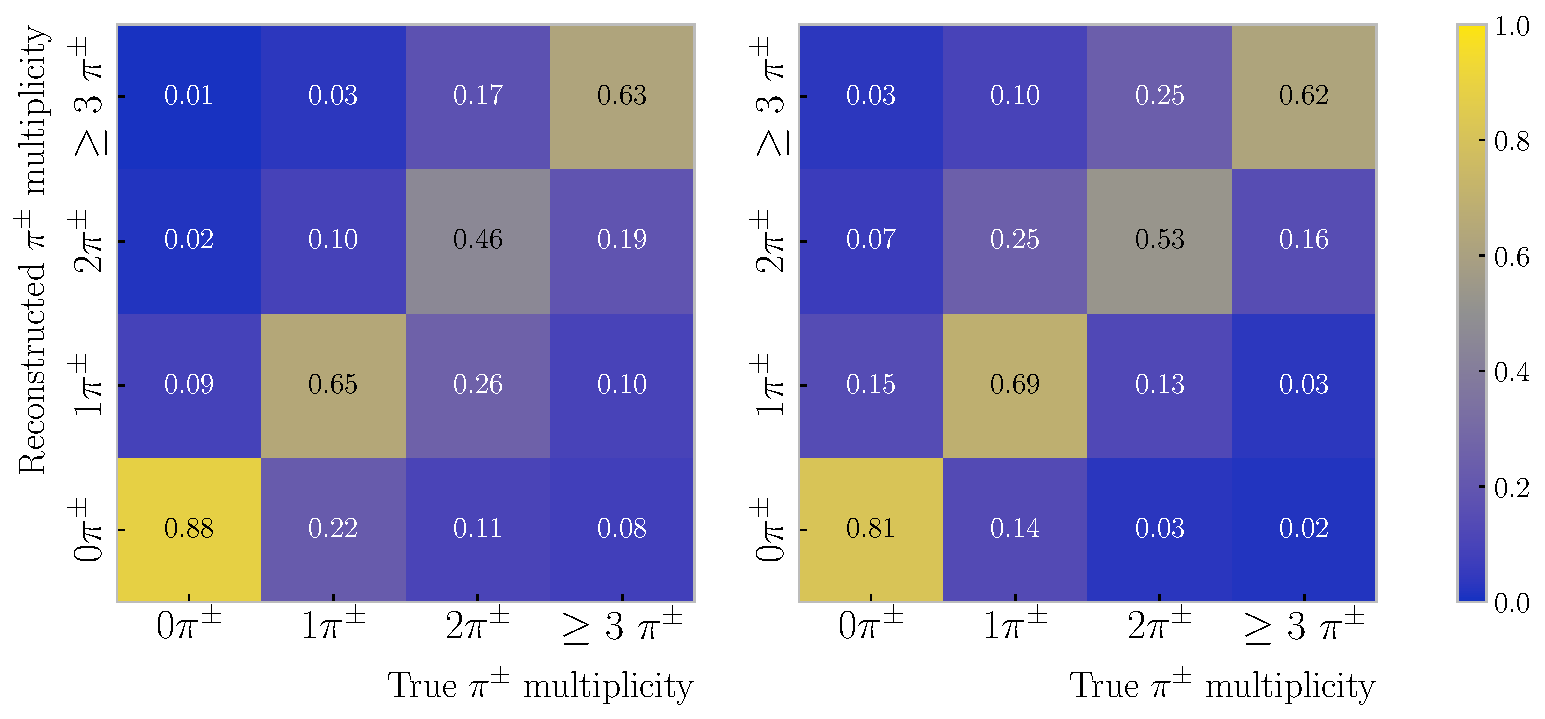
\includegraphics[width=.99\linewidth]{Images/GAr_selection/pion_selection_metrics_matrix_max_significance.pdf}
    \caption[Row and column normalised distributions of events given their true and reconstructed $\pi^{\pm}$ multiplicity, for the selection that maximises the significance of the $\nu_{\mu}$ CC $1\pi^{\pm}$ selection.]{Distribution of events given their true and reconstructed $\pi^{\pm}$ multiplicity, both column-wise (left panel) and row-wise (right panel) normalised, for the selection that maximises the significance of the $\nu_{\mu}$ CC $1\pi^{\pm}$ selection. The column normalisation yields the efficiency in the diagonal entries, whereas the row normalisation reveals the purity.}
    \label{fig:pion_selection_metrics}
\end{figure}

To have a working point for our studies, I chose the cut configuration that yields the maximum significance for the $\nu_{\mu}$ CC $1\pi^{\pm}$ selection. Of course, other cuts would be more appropriate in certain scenarios. However, this provides us with a starting point to understand the performance of the selection. A significance of $66\pm7$ for the $1\pi^{\pm}$ selection is achieved for the cut values $p^{\mathrm{cut}}_{\mathrm{d}E/\mathrm{d}x} = 0.30$, $p^{\mathrm{cut}}_{\mathrm{ToF}} = 0.70$, $\Delta^{\pi^{\pm}}_{\mathrm{d}E/\mathrm{d}x} = 0.10$, and $d^{\mathrm{cut}}_{\mu} = 110.0~\mathrm{cm}$.

Figure \ref{fig:pion_selection_metrics} shows the multiplicity matrices resulting from this optimised $\nu_{\mu}$ CC $1\pi^{\pm}$ selection. Although both matrices are produced with the same selection cuts, one is column normalised (left panel), whereas the other is row normalised (right panel). It follows from the definitions in Eqs. (\ref{eq:efficiency_matrix}) and (\ref{eq:purity_matrix}) that the diagonal entries of these matrices correspond to the efficiencies and the purities, respectively, for each of the possible charged pion multiplicity selections.

\begin{figure}[t]
    \centering
    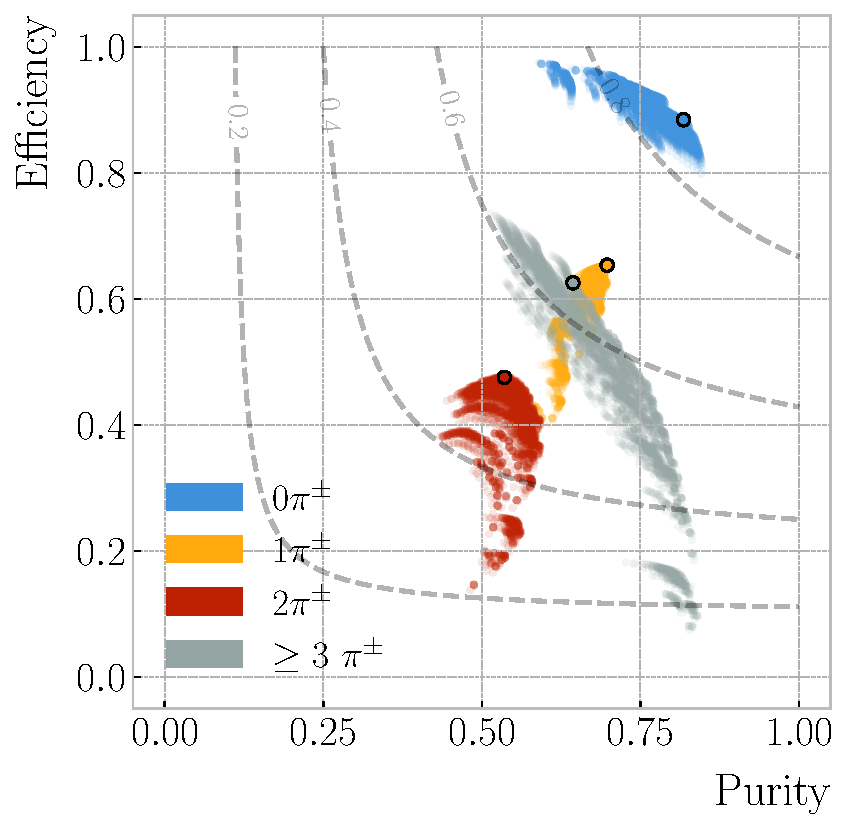
\includegraphics[width=.70\linewidth]{Images/GAr_selection/pion_selection_all_in_one_purity_vs_efficiency.pdf}
    \caption[Purity versus efficiency achieved for the different cut configurations explored separated by the various $\nu_{\mu}$ CC $N\pi^{\pm}$ selections.]{Purity versus efficiency achieved for the different cut configurations explored separated by the various $\nu_{\mu}$ CC $N\pi^{\pm}$ selections. The outlined points indicate the state for each possible multiplicity when using the configuration that maximises the significance of the $\nu_{\mu}$ CC $1\pi^{\pm}$ selection. The contours indicate the surfaces of equal $F_{1}$-score.}
    \label{fig:pion_purity_vs_efficiency}
\end{figure}

An additional check to make is understand how this configuration performs when applied to the other selections, like $\nu_{\mu}$ CC $0\pi^{\pm}$, and how it compares to the other possible configurations. A comparison between the different pion multiplicity selections, indicated with colours, in the purity versus efficiency space is shown in Fig. \ref{fig:pion_purity_vs_efficiency}. For each of the possible multiplicity choices, the performance obtained for the $1\pi^{\pm}$ optimised selection is indicated by an outlined point. From this, one can see that the selected configuration performs reasonably well, within the limits of what can be achieved in each case, across the different multiplicities.

\begin{figure}[t]
    \centering
    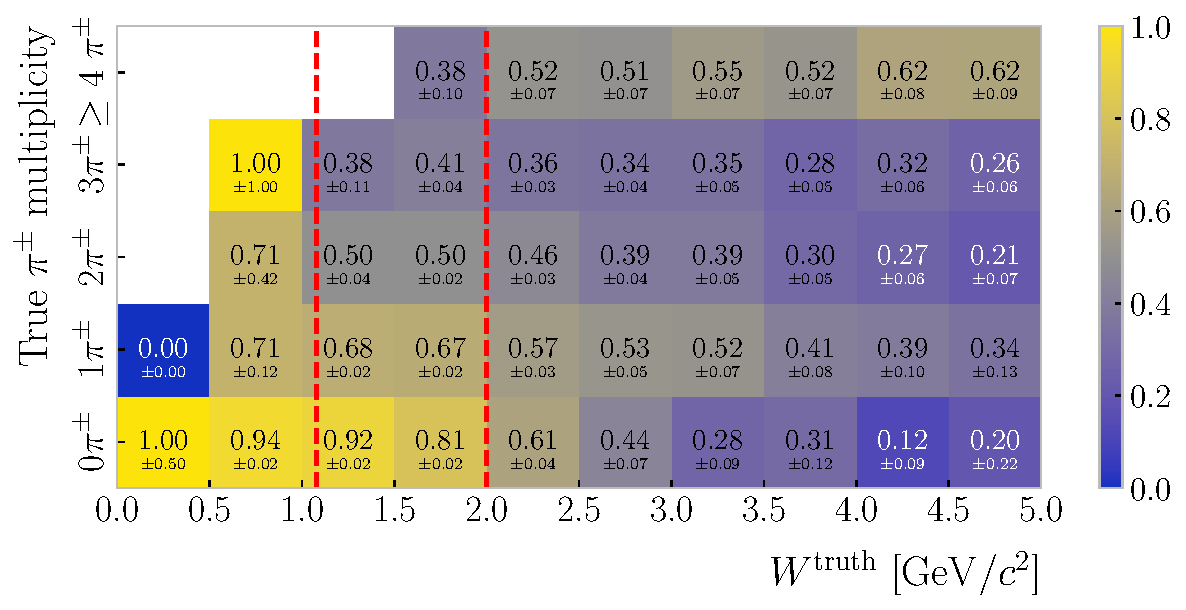
\includegraphics[width=.90\linewidth]{Images/GAr_selection/pion_selection_efficiency_versus_invariant_mass.pdf}
    \caption[Efficiency of the $\nu_{\mu}$ CC $N\pi^{\pm}$ selections as a function of the hadronic invariant mass.]{Efficiency of the various $\nu_{\mu}$ CC $N\pi^{\pm}$ selections as a function of the true hadronic invariant mass. The dashed vertical lines correspond (from left to right) to the values $m_{p}+m_{\pi^{\pm}}$ and $2.0~\mathrm{GeV}/c^{2}$, which define the shallow inelastic scattering region.}
    \label{fig:efficiency_vs_invariant_mass}
\end{figure}

At this point, one can study the charged pion selection performance as a function of other quantities of interest. A natural variable to check is the hadronic invariant mass. It is defined as:
\begin{equation}
W = \sqrt{-Q^{2} + 2 m_{n} q_{0} + m_{n}^{2}}
\end{equation}
where $Q^{2}$ is the momentum transfer from the neutrino to the primary muon, $q_{0}$ the energy transfer, and $m_{n}$ the mass of the nucleon. This quantity is related to the elasticity of the neutrino interaction, and defines the transitions between the QE, RES and DIS regions. An interesting invariant mass range for DUNE is the one that extents between the mass of the $\Delta$ resonance, even though thi is typically extended down to $m_{p}+m_{\pi^{\pm}}$, and $2.0~\mathrm{GeV}$. It is estimated that roughly $7$ in every $10$ events in our ND will take place in this region. Although the RES production dominates at these $W$ values, this range also includes the transition to the DIS regime. Thus, it is often called the shallow inelastic scattering (SIS) region.

Within these boundaries, the resonant events produce either $1$ or $2$ charged pions, whereas the multipion events are typically associated to non-resonant production. Therefore, our ability of correctly select events with $\geq 2\pi^{\pm}$ in the SIS region will impact our ability of constraining this poorly understood regime. Figure \ref{fig:efficiency_vs_invariant_mass} shows the efficiency of the various charged pion multiplicity selections in a number of hadronic invariant mass bins. The two red dashed lines indicate the boundaries of the SIS region. One can see that, although not as good as the single pion selection, the efficiency for the multipion events is reasonable in the relevant invariant mass range. The total efficiency for the $\nu_{\mu}$ CC $\geq 2\pi^{\pm}$ selection in the SIS regime is estimated to be $0.65 \pm 0.02$.

\subsection[\texorpdfstring{$\nu_{\mu}$}{numu} CC \texorpdfstring{$1\pi^{\pm}$}{1pi} selection]{\boldmath\texorpdfstring{$\nu_{\mu}$}{numu} CC \boldmath\texorpdfstring{$1\pi^{\pm}$}{1pi} selection}

By focusing on the $1\pi^{\pm}$ selection, one can study the kinematics of the selected pion. This allows to understand how well the charged pions are tagged. This is difficult to do only using the multiplicity matrices, as with them one can only check that the number of charged pions is the same as in the truth. Sometime, even if the estimated pion multiplicity is correct, the identified particles may not be true pions.

\begin{figure}[t]
    \centering
    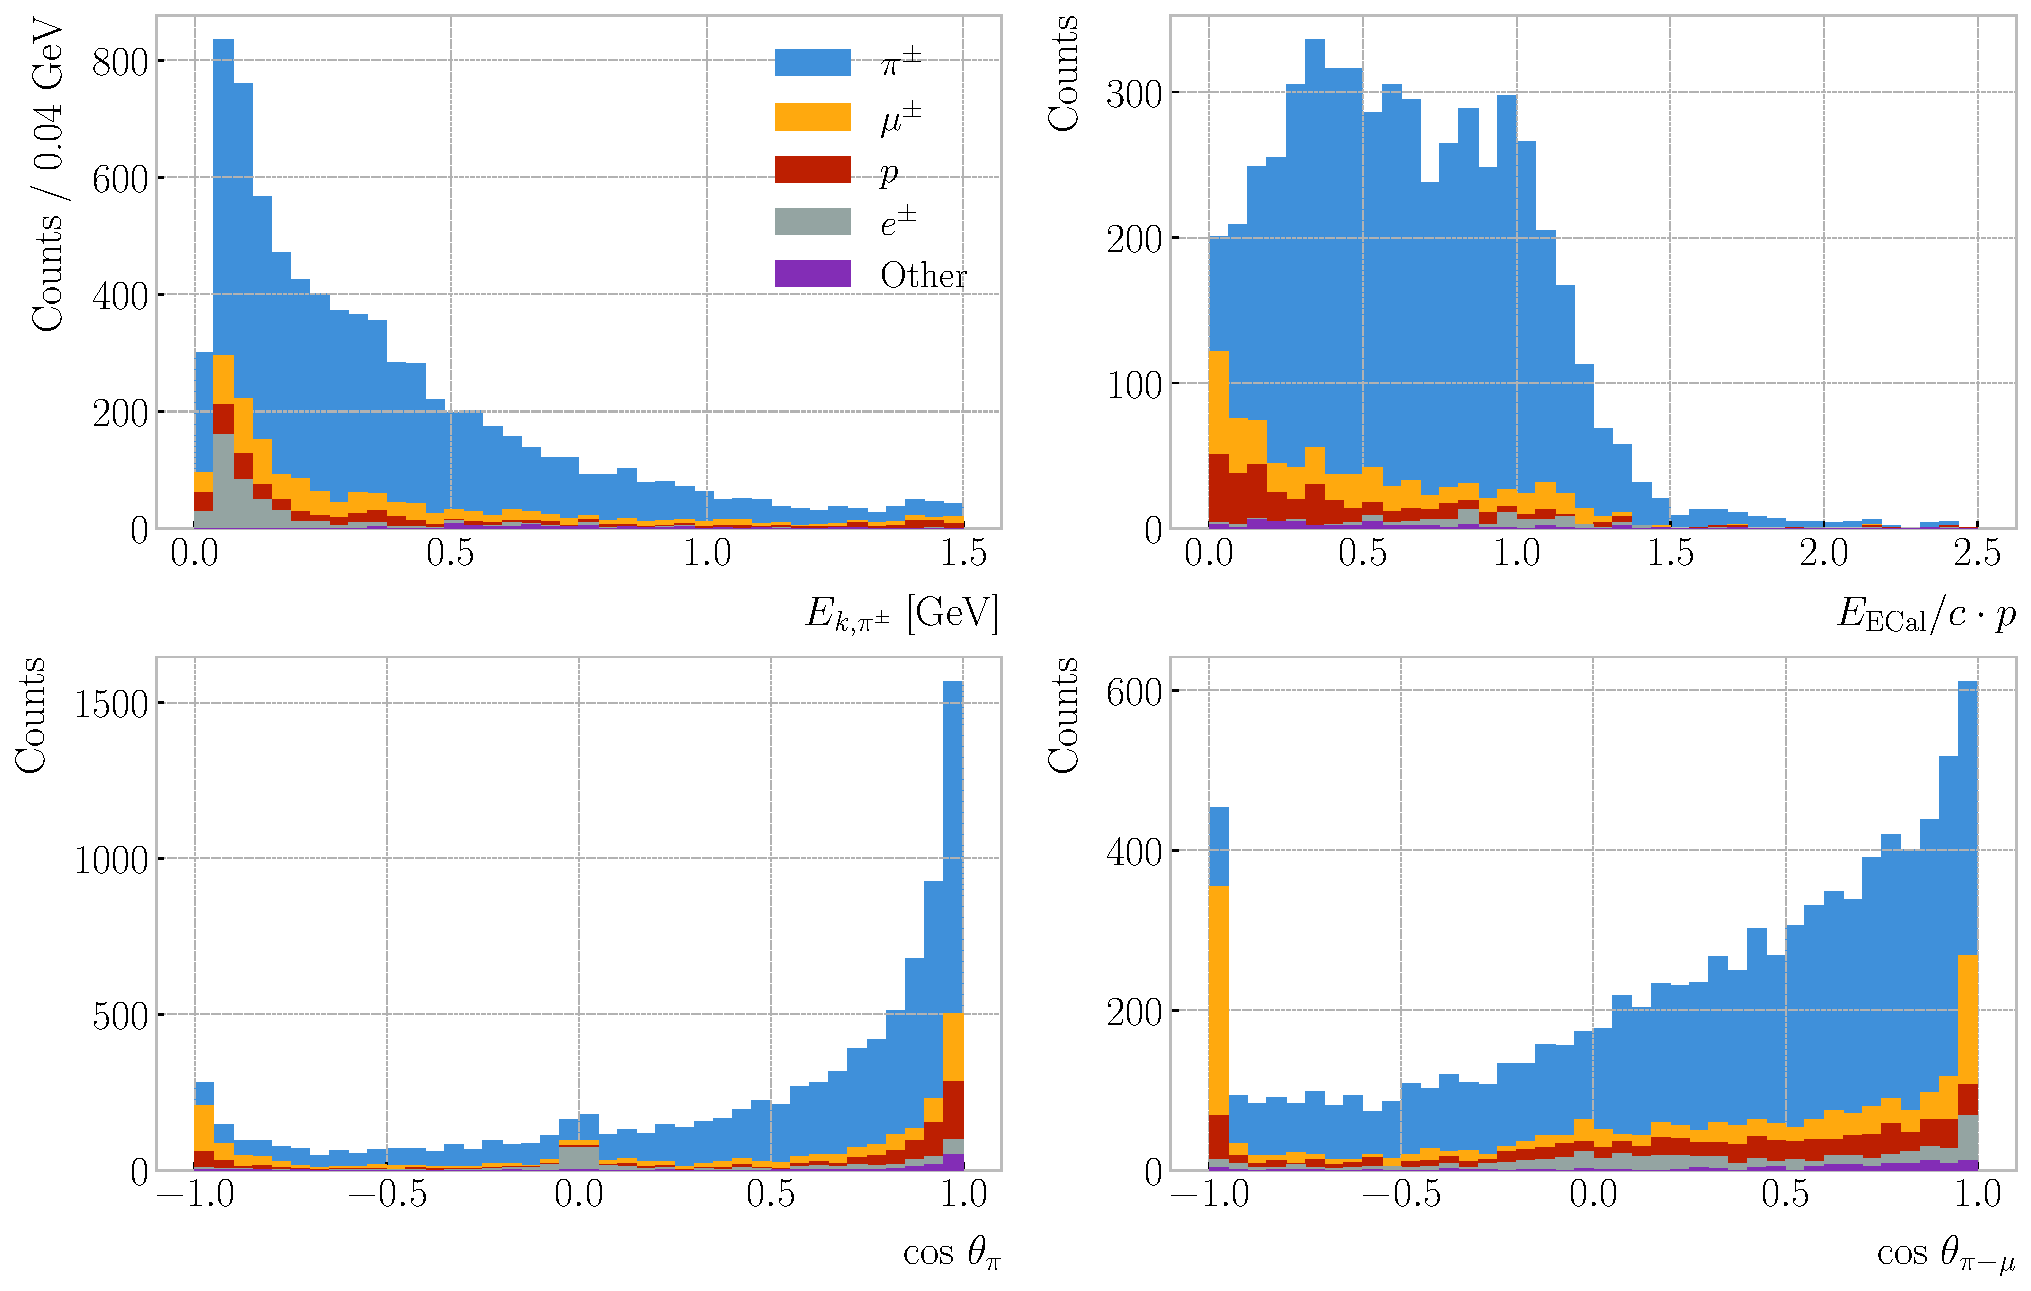
\includegraphics[width=.99\linewidth]{Images/GAr_selection/pion_selection_1pion_kinematics.pdf}
    \caption[Reconstructed kinematic distributions for the pion candidate in the $\nu_{\mu}$ CC $1\pi^{\pm}$ selection.]{Reconstructed kinematic distributions for the pion candidate in the $\nu_{\mu}$ CC $1\pi^{\pm}$ selection, broken down by true ID of the particle. From left to right, top to bottom, we have the kinetic energy given the pion hypothesis, the ratio between the energy deposited in the ECal and the momentum, the pion angle, and the angle between the muon and pion candidates.}
    \label{fig:1pion_kinematics}
\end{figure}

Figure \ref{fig:1pion_kinematics} displays the distributions of various reconstructed kinematic variables for the selected pion candidate. The different colours indicate the ID of the true particle associated to the reconstructed pion candidate.

First, we have the kinetic energy distribution. For this set of reconstructed particles, because they have been tagged as charged pions, the kinetic energy is computed using their momentum assuming the pion hypothesis. One can see that most of the contaminants sit in low energy range, up to around $0.2~\mathrm{GeV}$.

The next distribution presents the ratio between the energy deposited in the ECal associated to the particle over the momentum measured in the HPgTPC. This variable is restricted to particles with at least one associated hit in the ECal. It is interesting to see two peak structure in the true pion distribution. The first one presumably corresponds to the pions punching-through the ECal, while the latter is probably due to the ones stopping in it. On the other hand, the misidentified particles, other than the electrons, tend to lower ratios. This is expected for protons, as this could not be higher than $0.5$ for momenta $\leq 1~\mathrm{GeV}/c$ even if they stopped, but for the muons it may point to a misreconstruction problem.

\begin{figure}[t]
    \centering
    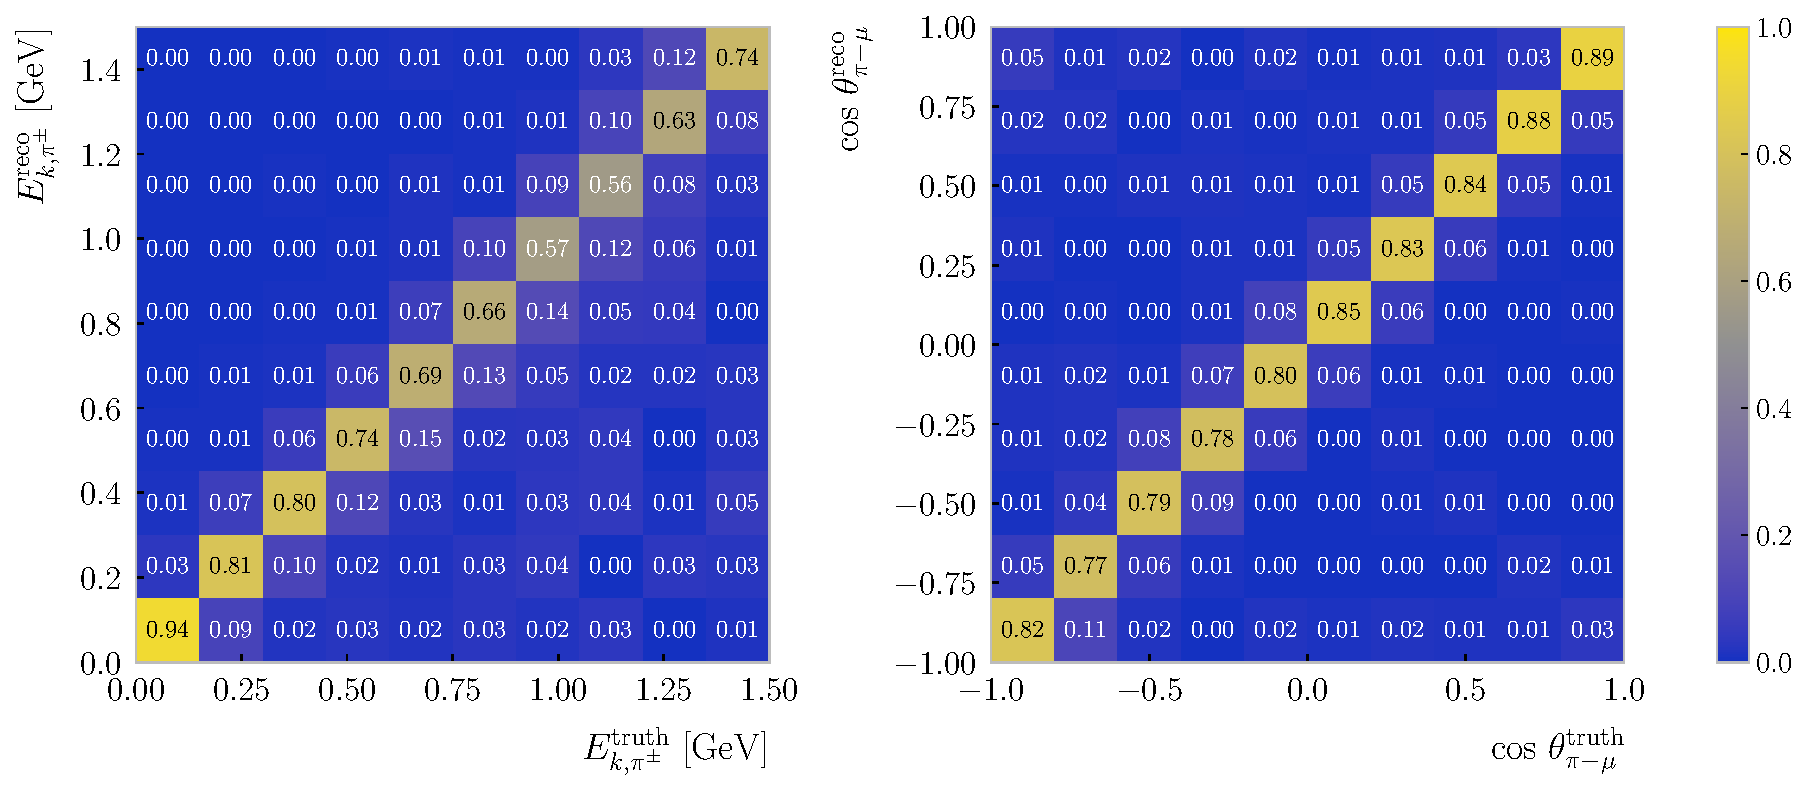
\includegraphics[width=.99\linewidth]{Images/GAr_selection/pion_selection_1pion_kinematic_comp.pdf}
    \caption[Distributions for the reconstructed versus truth pion kinetic energy and angle between the pion and muon in the $\nu_{\mu}$ CC $1\pi^{\pm}$ selection.]{Distributions for the reconstructed versus truth generated pion kinetic energy (left panel) and cosine of the angle between the pion and muon (right panel). The reconstructed values correspond to the selected primary muon and pion candidates in the $\nu_{\mu}$ CC $1\pi^{\pm}$ selection, whereas the truth values come from the true primary muon and pion in the events.}
    \label{fig:1pion_kinematic_comp}
\end{figure}

The following distribution shows the angle of the pion candidates with respect to the beam direction. Although most of them are aimed in the forward direction, it can be noted that an important number of the misidentified muons seem to be backward-going. This is likely a reconstruction artifact, produced by broken tracks that got assigned the wrong propagation direction. Also, there is a sizeable number of true electrons with directions perpendicular to the beam, probably delta electrons from the primary muon.

Finally, I included the reconstructed pion-muon angular distribution. Even though it shares some similarities with the previous distribution, as the primary muon typically goes forward, the pion distribution is not as prominently forward-going in this case. Also, it may be noted that approximately $25\%$ of the muons misidentified as pions have $\mathrm{cos}~\theta_{\pi - \mu} \leq -0.95$. Therefore, putting an additional angular cut improves the purity of the charged pion selection from $0.74 \pm 0.01$ to $0.77 \pm 0.01$, while not loosing a substantial amount of true pions.

A comparison between the true and the reconstructed values of the pion kinetic energy (left panel) and pion-muon angle (right panel) is shown in Fig. \ref{fig:1pion_kinematic_comp}. The distributions are column normalised, which allows to see the fraction of events in the correct bins. For this, I select the events where only one reconstructed pion and one true pion were identified, as that is the only case were a pairing of the variables is possible. It showcases the excellent agreement between the reconstruction and the truth information.

\begin{figure}[t]
    \centering
    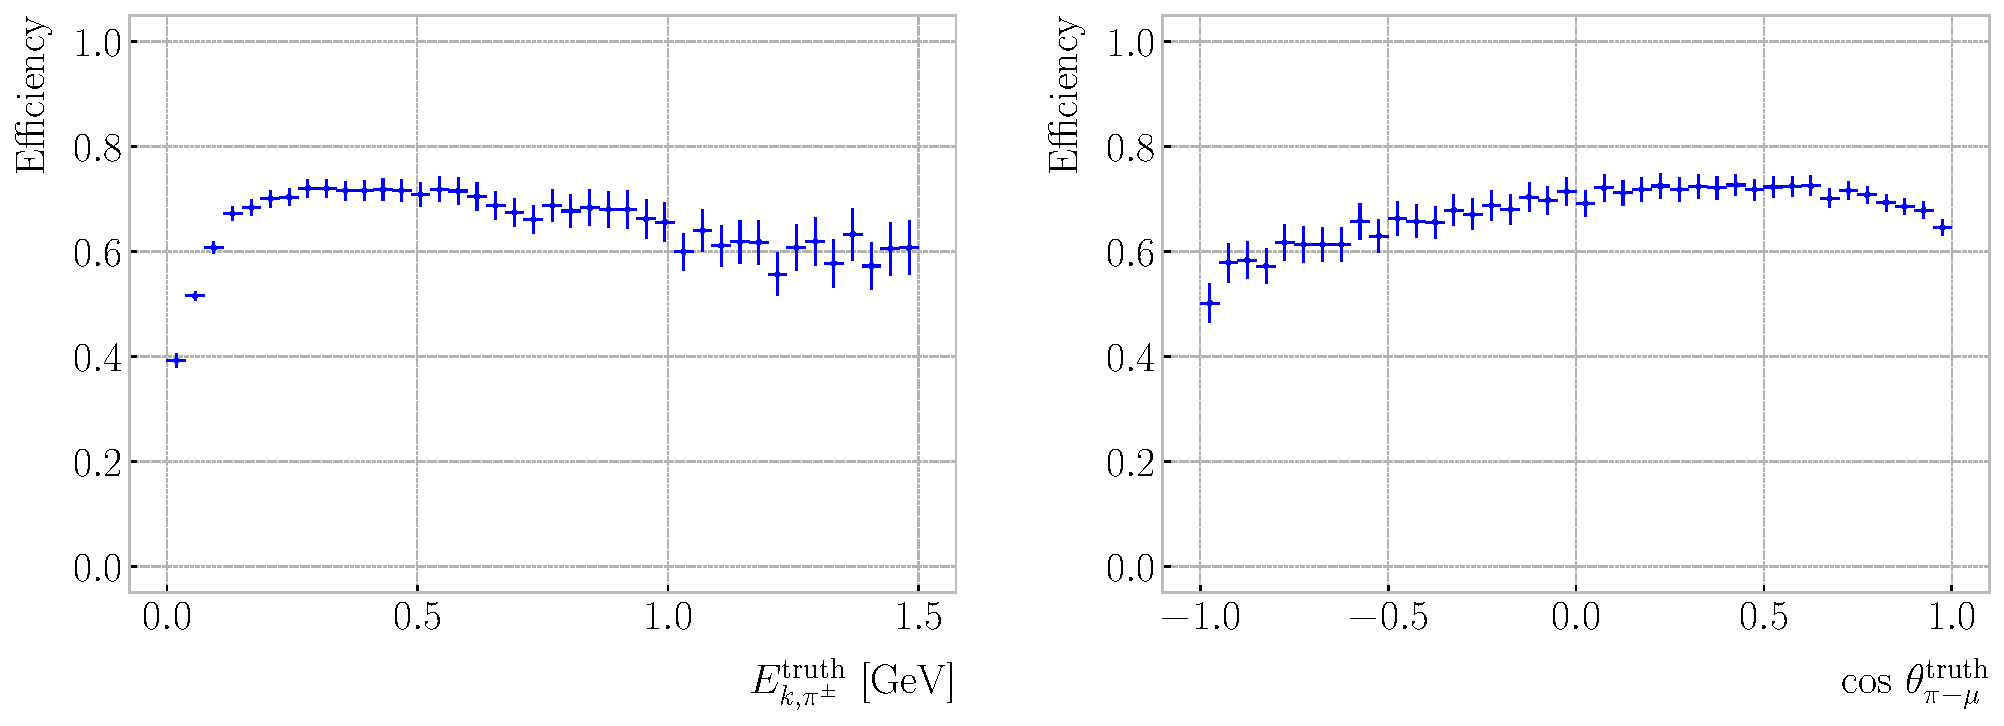
\includegraphics[width=.99\linewidth]{Images/GAr_selection/pion_selection_1pion_kin_efficiency.pdf}
    \caption[Efficiency of the $\nu_{\mu}$ CC $1\pi^{\pm}$ selection as a function of the true pion kinetic energy and pion-muon angle.]{Efficiency of the $\nu_{\mu}$ CC $1\pi^{\pm}$ selection as a function of the true pion kinetic energy (left panel) and pion-muon angle (right panel).}
    \label{fig:1pion_kin_efficiency}
\end{figure}

One can also study the performance of the pion selection as a function of the truth pion kinematics. Fig. \ref{fig:1pion_kin_efficiency} shows the selection efficiency versus the true kinetic energy (left panel) and the angle between the true primary pion and muon (right panel). The efficiency is computed from the events with a single true and reconstructed pion, comparing their number to the total of events with one true pion. Notice how the efficiency, although it starts with relatively low values, plateaus around $0.70$ quickly after $0.20~\mathrm{GeV}$. In terms of the pion-muon angle, the efficiency looks relatively flat, only dropping slightly towards the back-to-back case.

\section{Neutral pion identification}
\label{sec:gar_neutral_pions}

The $\nu_{\mu}$ CC selection can also be used as a stepping stone for the identification of neutral pions. Although these particles do not leave any traces in the HPgTPC, using a combination of the different detectors within ND-GAr they may be identified. Being able to tag the neutral pions is a valuable asset for the estimation of the reconstructed neutrino energy, as both their kinetic and mass components can then be added in the calculation.

In the case that both photons from the $\pi^{0}$ decay do not undergo pair production of a $e^{+}e^{-}$ pair, they will reach the ECal where they will produce an electromagnetic shower. This activity inside the ECal will not be associated to any charged particle track inside the HPgTPC, unless there is a reconstruction failure. Thus, having a neutrino interaction vertex candidate from the $\nu_{\mu}$ CC selection, one can reconstruct the mass of the $\pi^{0}$ using the energy and position of the photons. I already used this same technique in section \ref{section:neutral} for a single $\pi^{0}$ sample. However, here I apply it to neutrino interaction events, and the vertex position is not cheated but selected from the reconstruction products.

The idea is to look for all the ECal clusters that were not associated to tracks in each event. Then, if two or more were identified, compute the invariant mass for all possible combinations. At this point, I select the pair whose invariant mass is closest to $m_{\pi^{0}}$, remove the pairs containing any of the two selected clusters from the collection, and iterate until no more pairs can be formed.

I repeat this procedure for the events with $0$, $1$, $2$ and $3$ or more true neutral pions. For each of them, I extract the invariant mass of the first three cluster pair candidates (in order of proximity to $m_{\pi^{0}}$), in case they can be formed. If the number of the cluster pair is lower than the true neutral pion multiplicity of the event, that entry will be counted as signal. The additional candidates for an event of a given multiplicity are considered background. The resulting distribution is shown in Fig. \ref{fig:pizero_invariant_mass} (black data points).

I fit the signal distribution to a double-sided Crystal Ball function:
\begin{equation}
    f_{s} (x; ~\alpha_{L,R}, n_{L,R}, \mu, \sigma, N) = N \left\{
    \begin{array}{ll}
        A_{L} \left(B_{L} - \frac{x - \mu}{\sigma}\right)^{-n_{L}}, & \mathrm{for} \ \frac{x - \mu}{\sigma} < -\alpha_{L},\\
        \mathrm{e}^{-\frac{(x-\mu)^{2}}{2 \sigma^{2}}}, & \mathrm{for} \ -\alpha_{L} \leq \frac{x - \mu}{\sigma} \leq \alpha_{R},\\
        A_{R} \left(B_{R} + \frac{x - \mu}{\sigma}\right)^{-n_{R}}, & \mathrm{for} \ \frac{x - \mu}{\sigma} > \alpha_{R},
    \end{array}
    \right.
\end{equation}
where $A_{L,R}$ and $B_{L,R}$ are given by:
\begin{equation}
\begin{split}
    A_{L,R} &= \left(\frac{n_{L,R}}{|\alpha_{L,R}|}\right)^{n_{L,R}} \mathrm{e}^{-\frac{|\alpha_{L,R}|^{2}}{2}},\\
    B_{L,R} &= \frac{n_{L,R}}{|\alpha_{L,R}|}-|\alpha_{L,R}|.
\end{split}
\end{equation}
The tails of this distribution accommodate the asymmetric shape dut to the misreconstruction effects. The values obtained for the best fit parameters are indicated in Fig. \ref{fig:pizero_invariant_mass} (blue box).

\begin{figure}[t]
    \centering
    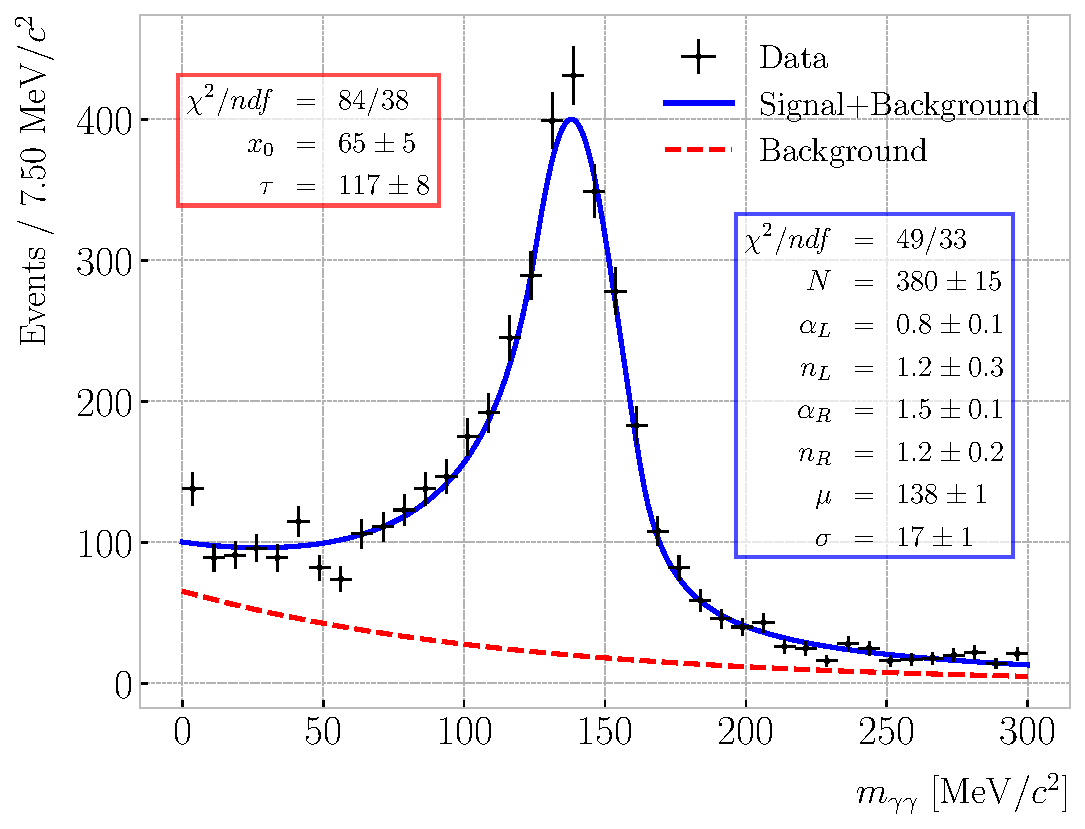
\includegraphics[width=.80\linewidth]{Images/GAr_selection/numuCC_1pizero_selection.pdf}
    \caption[Invariant mass distribution obtained for the unassociated ECal cluster pairs in the event.]{Invariant mass distribution obtained for the unassociated ECal cluster pairs in the event. The best fits for signal plus background (solid blue line) and background only (dashed red line) are also shown.}
    \label{fig:pizero_invariant_mass}
\end{figure}

The background is characterised by an exponential function of the form:
\begin{equation}
    f_{b} (x; ~x_{0}, \tau) = x_{0} \mathrm{e}^{-x/\tau}.
\end{equation}
Similarly, the best fit values can be seen in Fig. \ref{fig:pizero_invariant_mass} (red box).

Figure \ref{fig:pizero_invariant_mass} also shows the results of the fits for the signal plus background (blue line) and the background only (dashed red line) cases. Using these, I estimate the tagging efficiency of this method to be $0.90 \pm 0.01$ with a purity of $0.85 \pm 0.01$, when selecting the candidates with an invariant mass in the range $54.0-288.0~\mathrm{GeV}/c^{2}$.

This is a robust method to identify the photon pair from the $\pi^{0}$ decay. However, this approach is not enough to efficiently identify all the events containing neutral pions in the sample. A quick calculation reveals that only $20\%$ of the $\nu_{\mu}$ CC $1\pi^{0}$ events can be correctly identified with it.

This approach can be complemented with the identification of the secondary vertices from the $e^{+}e^{-}$ conversions. This will make it possible to cover the cases when either one or both photons convert in the HPgTPC. In those cases, one can try pairing the $e^{+}e^{-}$ with unassociated activities in the ECal, or matching pairs of secondary vertices. However, this will require further work on the reconstruction, and thus falls out of the scope of this analysis.

\section{Neutrino energy reconstruction}
\label{sec:gar_energy}

In a neutrino-nucleus CC interaction, where alongside the charged lepton $N$ nucleons where knocked out and $M$ mesons produced, the reconstructed neutrino energy can be computed as:
\begin{equation}
    E_{\mathrm{rec}} = S_{n} + E_{\ell} + \sum_{i=0}^{N} E_{k,n_{i}} + \sum_{j=0}^{M} E_{m_{j}},
\end{equation}
where $S_{n}$ is the average single-nucleon separation energy, $E_{\ell}$ the energy of the primary lepton, $E_{k,n_{i}}$ is the kinetic energy of the $i$-th knocked-out nucleon and $E_{m_{j}}$ the total energy of the $j$-th produced meson.

This represents the ideal scenario, where all the kinetic energy of the nucleons is visible in the detector and one can identify all mesons produced in the interaction. In a real experiment, some of these energy components will be missed, and this needs to be accounted for in any estimation of the reconstructed energy.

For instance, in ND-GAr neutrons are complicated to account for, as they do not produce tracks in the TPC. They may be identified either from scatterings off Ar nuclei in the HPgTPC, or performing a ToF measurement in the ECal. However, these methods are not fully mature in the current reconstruction, and their development is beyond the scope of this study. So, in the following, I will completely ignore the contribution of neutrons.

Also, with a real detector we can not expect to tag all the charged pions irrespective of their energy. This is why one has to introduce detection thresholds in the energy estimation. Thus, in the reconstructed energy calculation I will add only the kinetic energy for the charged pions below the threshold, and the total energy for the  pions above the threshold.

Likewise, the identification of all neutral pions in the sample is challenging. As discussed in the previous section, with our ECal we are able to identify the photons from the $\pi^{0}$ decays, but that selection still needs to be completed with other methods. Therefore, for this first study I do not take into account the energy contribution of the neutral pions.

With all this in mind, using the truth information from the events I compute the reconstructed neutrino energy as:
\begin{equation}
    E^{\mathrm{truth}}_{\mathrm{rec}} = S_{n} + E_{\ell} + \sum_{i=0}^{N_{p}} E_{k,p_{i}} + \sum_{j=0}^{M_{\pi^{\pm}}^{<}} E_{k,\pi^{\pm}_{j}} + \sum_{k=0}^{M_{\pi^{\pm}}^{\geq}} E_{\pi^{\pm}_{k}},
\end{equation}
where $N_{p}$ is the number of protons, and $M_{\pi^{\pm}}^{<}$ and $M_{\pi^{\pm}}^{\geq}$ the number of charged pions below and above the threshold, respectively. As before, I assume a kinetic energy threshold of $20~\mathrm{MeV}$ for the charged pions.

At the reconstruction level, I use the energy of the primary muon candidate, computed from its momentum, as the starting point for the neutrino energy calculation. Then, I add the total energy contributions from the identified charged pions, again using their momenta. After that, I try to identify the protons by looking at the two proton scores. If any of them are above threshold (here the thresholds used are the same as for the pion identification), the kinetic energy of the particle is added to the total. Finally, I check if any of the remaining particles are fully contained within the FV. I add their kinetic contributions using the total energy they deposited in the HPgTPC.

\begin{figure}[t]
    \centering
    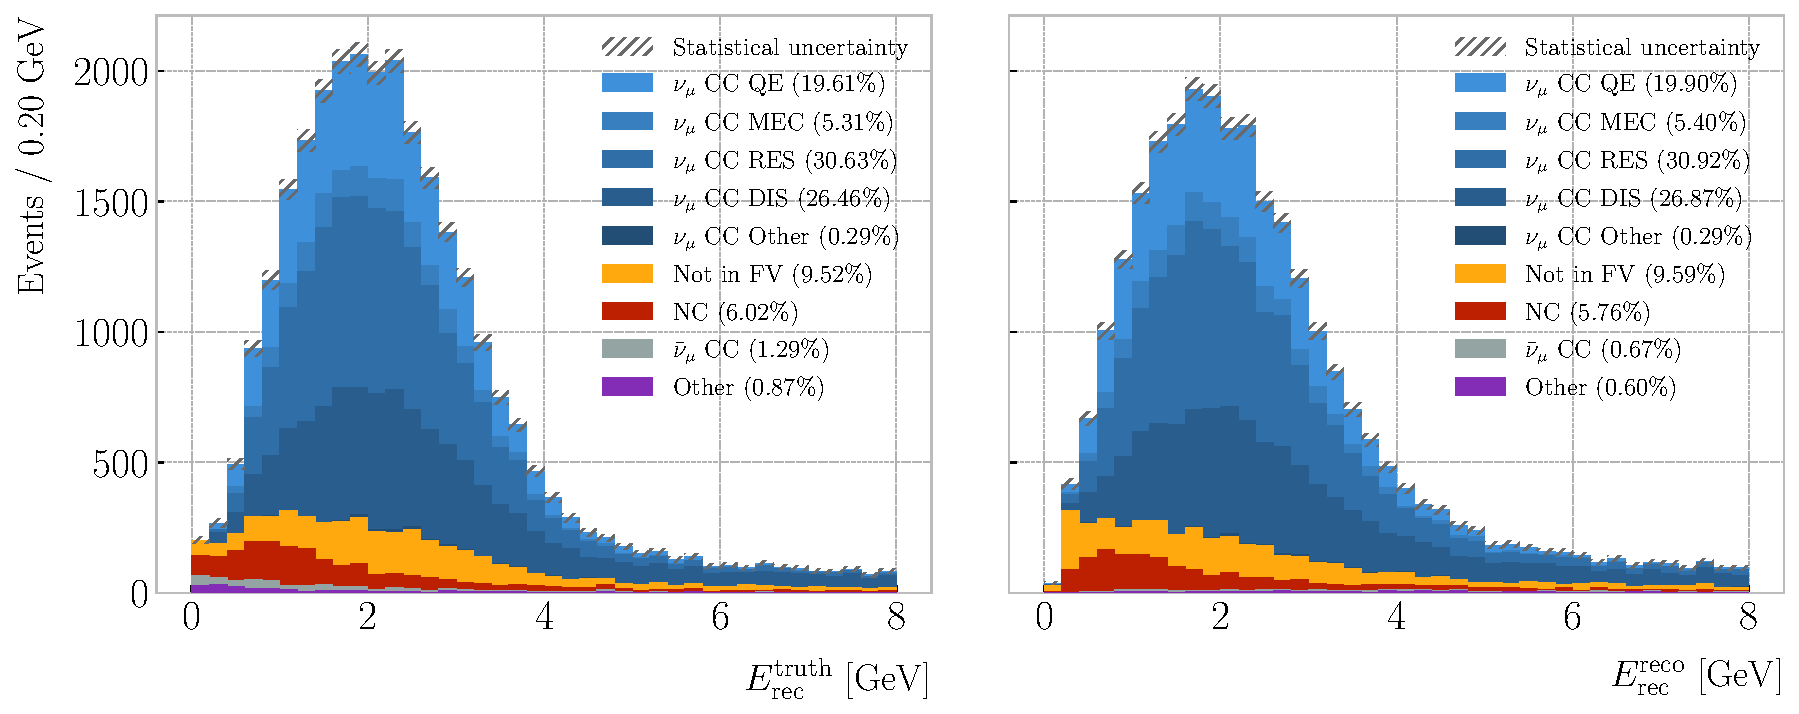
\includegraphics[width=.99\linewidth]{Images/GAr_selection/numuCC_selection_reco_energy_comparison.pdf}
    \caption[Reconstructed neutrino energy spectra for the $\nu_{\mu}$ CC selection obtained using the truth and reconstructed information]{Reconstructed neutrino energy spectra for the $\nu_{\mu}$ CC selection obtained using the truth (left panel) and reconstructed (right panel) information. The selected events are broken down by signal and background subcategories. The statistical uncertainty is drawn in hatched gray.}
    \label{fig:numuCC_reconstructed_energy}
\end{figure}

Figure \ref{fig:numuCC_reconstructed_energy} shows the resulting distributions of reconstructed neutrino energy obtained from the truth (left panel) and reconstructed (right panel) particle collections. The overall shape of the distributions is similar, with the reconstructed one having a slightly larger high energy tail. Note also that the background events from outside the FV tend to have a smaller energy in the reconstructed case. This is likely due to a misreconstruction of the primary muon, which clearly does not affect the other computation.

I also compared the reconstructed energies to the true energy of the neutrino. Figure \ref{fig:numuCC_reconstructed_fresiduals} displays the ratio of the energy residuals to the true energy for the truth (left panel) and reconstructed (right panel) cases. As expected, using the true particles one never overestimates the neutrino energy. Also, using the reconstructed objects one is more prone to underestimate the neutrino energy, due to deficiencies in the reconstruction.

\begin{figure}[t]
    \centering
    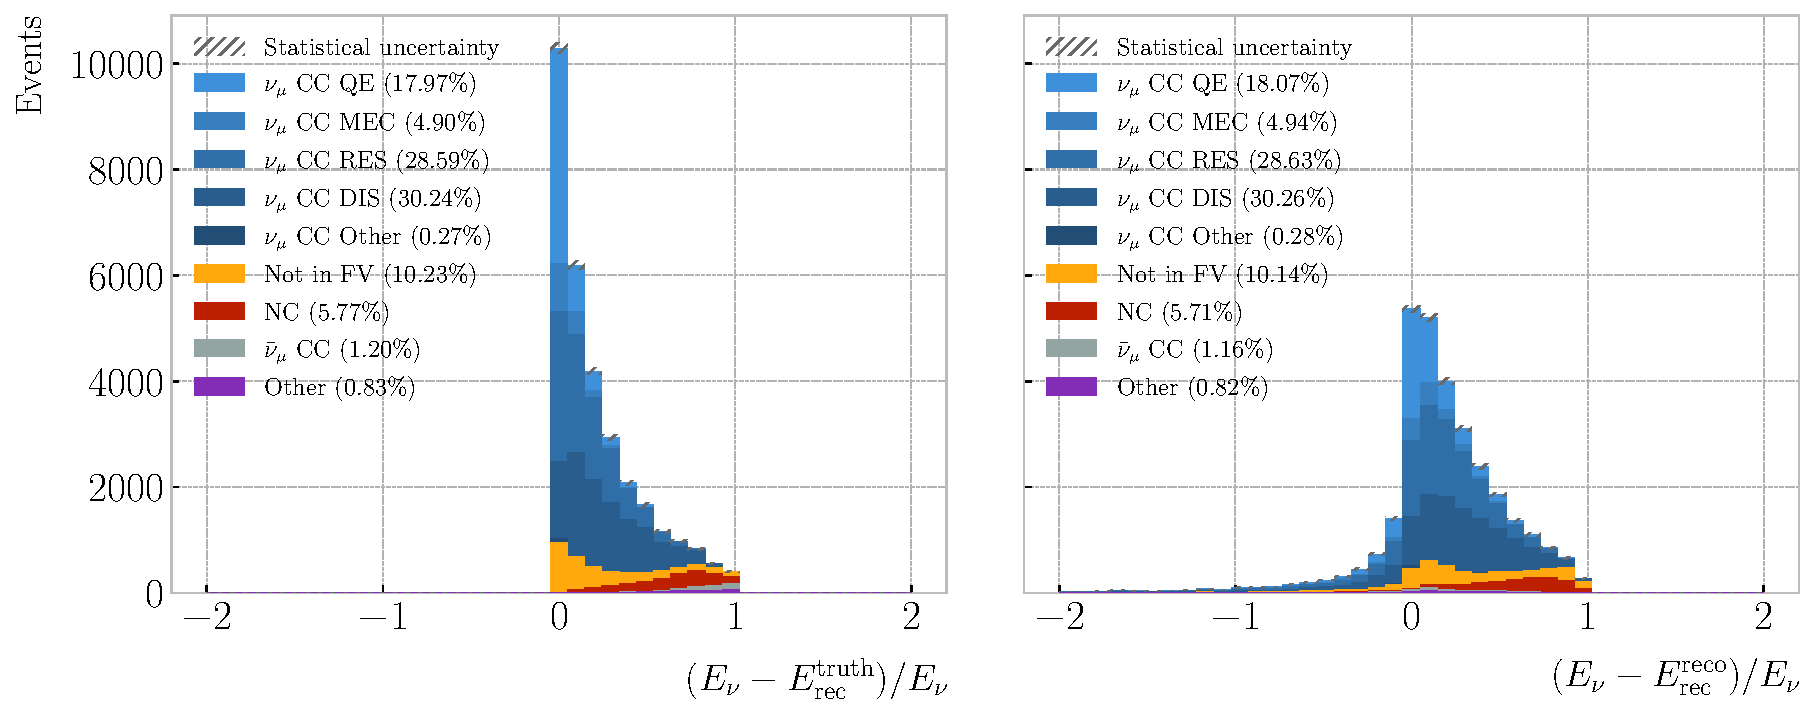
\includegraphics[width=.99\linewidth]{Images/GAr_selection/numuCC_selection_truth_reco_energy_fresiduals_comparison.pdf}
    \caption[Neutrino energy residuals distributions for the $\nu_{\mu}$ CC selection obtained using the truth and reconstructed information]{Neutrino energy residuals distributions for the $\nu_{\mu}$ CC selection obtained using the truth (left panel) and reconstructed (right panel) information. The selected events are broken down by signal and background subcategories. The statistical uncertainty is drawn in hatched gray.}
    \label{fig:numuCC_reconstructed_fresiduals}
\end{figure}

\section{Systematic uncertainties}
\label{sec:gar_systematics}

Although the implementation and study of the systematic uncertainties relevant for ND-GAr is out of the scope of this preliminary analysis, in this section I give an extended overview of the topic. These can be classified in three categories: neutrino flux uncertainties, neutrino-nucleus interaction model uncertainties, and detector response uncertainties.

\subsection{Flux uncertainties}

% Introduction
The neutrino flux prediction is affected by systematic uncertainties arising from two sources: the uncertainties in the production of hadrons in the target and the uncertainties in the design parameters of the beamline itself. These fluxes and their uncertainties are generated with the G4LBNF simulation \cite{DUNE2020TDR2}, a Geant4 implementation of the LBNF beamline, and the Package to Predict the FluX (PPFX) framework, originally developed for MINERvA \cite{Golan2016}.

% Hadron-production uncertainties
The hadron production uncertainties are associated to the kinematic distributions of the hadrons produced when the protons interact with the carbon target, as well as the possible interactions of the hadrons with the beamline materials. The PPFX package estimates these uncertainties by performing a number of random throws of the production model parameters \cite{Bashyal2017}. This way, different predictions of the LBNF flux are generated, which can be compared to the nominal prediction to build a matrix of the covariances between neutrino energies, flavours and running modes (either FHC or RHC). The resulting hadron production uncertainties are described by the eigenvectors associated to the largest eigenvalues in this matrix, obtained performing a PCA analysis.

% Beamline instrumentation uncertainties
The other set of uncertainties affecting the neutrino flux prediction come from the limited precision with which we know the parameters of the different components in the beamline. These include the specifications of the target, the dimensions of the decay pipe, and the current and alignment of the magnetic horns. The effects on the flux predictions of these uncertainties are estimated using the G4LBNF simulation. For each of the parameters, the simulation runs with said parameter shifted by $\pm 1\sigma$ from the nominal value, and the resulting flux prediction is compared to the nominal one.

\subsection{Cross-section uncertainties}

As discussed previously in section \ref{sec:nu_interactions}, the neutrino-nucleus interaction model is of great importance for neutrino experiments, as it maps the true neutrino energy to the kinematics of the final state particles. The uncertainties on the cross-section model are implemented in three ways: varying the parameters used in the \texttt{GENIE} simulation, using weights that parametrise cross-section effects not accounted for in \texttt{GENIE}, and comparing the \texttt{GENIE} predictions to other interaction models.

Within the DUNE TDR LBL analysis, the default interaction model was that implemented in \texttt{GENIE} \texttt{v2_12_10} \cite{DUNE2021}. A summary of the cross section systematic parameters present in \texttt{GENIE} used in that analysis is presented in Tab. \ref{tab:xsec_genie_systs}. The additional systematic parameters used in the analysis are described in Tab. \ref{tab:xsec_non_genie_systs}.

\begin{table}[p!]
	\caption[Neutrino interaction systematic parameters implemented in \texttt{GENIE} used in the DUNE TDR LBL analysis.]{Neutrino interaction systematic parameters implemented in \texttt{GENIE} used in the DUNE TDR LBL analysis. Events with low $W$ that are not QE are mainly RES, whereas DIS events dominate at high $W$. The initials BY refer to the Bodek-Yang model. Table adapted from Ref. \cite{DUNE2021}.}
	\begin{center}
		\begin{small}
			\begin{tabular}{l|l}
                Systematic                                     & $1\sigma$ value                 \\[2mm] \hline
                \rule{0pt}{1.1\normalbaselineskip}\textbf{Quasielastic}                          &                                 \\[2mm]
                Axial mass for CCQE                            & $^{+0.25}_{-0.15}~\mathrm{GeV}$ \\[2mm]
                CCQE vector form factor shape                  & N/A                             \\[2mm]
                Fermi surface momentum for Pauli blocking      & $\pm 30\%$                      \\[2mm] \hline
                \rule{0pt}{1.1\normalbaselineskip}\textbf{Low $W$}                               &                                 \\[2mm]
                Axial mass for CC resonance                    & $\pm 0.05 ~ \mathrm{GeV}$       \\[2mm]
                Vector mass for CC resonance                   & $\pm 10\%$                      \\[2mm]
                $\theta_{\pi}$ distribution for $\Delta$ decay & N/A                             \\[2mm] \hline
                \rule{0pt}{1.1\normalbaselineskip}\textbf{High $W$ (BY model)}                   &                                 \\[2mm]
                $A_{\mathrm{HT}}$                              & $\pm 25\%$                      \\[2mm]
                $B_{\mathrm{HT}}$                              & $\pm 25\%$                      \\[2mm]
                $C_{v1u}$                                      & $\pm 30\%$                      \\[2mm]
                $C_{v2u}$                                      & $\pm 40\%$                      \\[2mm] \hline
                \rule{0pt}{1.1\normalbaselineskip}\textbf{Other neutral current}                 &                                 \\[2mm]
                Axial mass for NC resonance                    & $\pm 10\%$                      \\[2mm]
                Vector mass for NC resonance                   & $\pm 5\%$                       \\[2mm] \hline
                \rule{0pt}{1.1\normalbaselineskip}\textbf{Intra-nuclear}                         &                                 \\[2mm]
                Nucleon charge exchange                        & $\pm 50\%$                      \\[2mm]
                Nucleon elastic reaction                       & $\pm 30\%$                      \\[2mm]
                Nucleon inelastic reaction                     & $\pm 40\%$                      \\[2mm]
                Nucleon absorption                             & $\pm 20\%$                      \\[2mm]
                Nucleon $\pi$-production                       & $\pm 20\%$                      \\[2mm]
                $\pi$ charge exchange                          & $\pm 50\%$                      \\[2mm]
                $\pi$ elastic reaction                         & $\pm 10\%$                      \\[2mm]
                $\pi$ inelastic reaction                       & $\pm 40\%$                      \\[2mm]
                $\pi$ absorption                               & $\pm 20\%$                      \\[2mm]
                $\pi$ $\pi$-production                         & $\pm 20\%$                     
            \end{tabular}
		\end{small}
	\end{center}
	\label{tab:xsec_genie_systs}
\end{table}

% Nuclear model
In this default \texttt{GENIE} configuration, the initial state of the nucleons is described by the Bodek-Ritchie global Fermi gas model \cite{Bodek1980}. The model is known to give a poor agreement when compared to neutrino-nucleon data \cite{Wilkinson2016}. Because of the limitations of the model, the current versions of \texttt{GENIE} use the local Fermi gas approach, which takes into account the correlation between the momentum of the nucleons and their location within the nucleus.

% CCQE
For the CCQE events, the dominant model uncertainties arise from the axial form factor of the nucleon, for which a dipole parametrisation is used, and the nuclear correlation effects computed using the random phase approximation (RPA). In the analysis, a parametrisation of the Valencia RPA effect \cite{Nieves2011} is used. This consists of a third-order Bernstein polynomial up to $Q^{2} = 1.2 ~ \mathrm{GeV}^{2}$ followed by an exponential decay (BeRPA), originally proposed by the T2K collaboration \cite{T2K2018}.

\begin{table}[t]
	\caption[Neutrino interaction systematic parameters used in the DUNE TDR LBL analysis not present in \texttt{GENIE}.]{Neutrino interaction systematic parameters used in the DUNE TDR LBL analysis not present in \texttt{GENIE}. I have omitted the parameters only relevant for the FD. Table adapted from Ref. \cite{DUNE2021}.}
	\begin{center}
		\begin{small}
			\begin{tabular}{l|l|l}
                Systematic         & Mode        & Description                         \\[2mm] \hline
                \rule{0pt}{1.1\normalbaselineskip}BeRPA              & $1p1h$/QE   & Nuclear model suppression           \\[2mm]
                ArC2p2h            & $2p2h$ Ar/C   & Electron scattering SRC pairs       \\[2mm]
                $E_{2p2h}$         & $2p2h$        & $2p2h$ energy dependence            \\[2mm]
                CC non-resonant    & CC DIS $1\pi$ & $\nu + n/p \rightarrow \ell + 1\pi$ \\[2mm]
                Other non-resonant & DIS $N\pi$    & $1 < W < 5 ~ \mathrm{GeV}/c^{2}$    \\[2mm]
                NC normalisation   & NC            & $\pm 20\%$ to all NC events at the ND
            \end{tabular}
		\end{small}
	\end{center}
	\label{tab:xsec_non_genie_systs}
\end{table}

% CCMEC (2p2h)
The $2p2h$ interactions are included using the Valencia model \cite{Nieves2011}, with an additional correction following the observation of an underprediction of these events in MINERvA \cite{MINERvA2015}. Additional uncertainties for the energy dependence of the missing strength were added. Also, the uncertainties in the scaling from carbon to argon are included, based on measurements of electron scattering off short-range correlated (SRC) nucleon pairs on multiple targets \cite{Colle2015}.

% CCRES
In this version of \texttt{GENIE}, the Rein-Sehgal model describes the single pion resonant production events \cite{Rein1980}. It includes 16 different resonances, with no interference between them. Two parameters account for the uncertainties on the axial and vector masses of the resonances. In subsequent \texttt{GENIE} tunes, like the one used in the studies presented in this Chapter, the Berger-Sehgal model is used \cite{Berger2007}. This is an improved version of the Rein-Sehgal model, which includes the lepton mass effects in the calculations.

% DIS (BY and NOvA)
The Bodek-Yang parametrisation is used to describe the DIS events \cite{Bodek2002}. The parameters $A_{\mathrm{HT}}$ and $B_{\mathrm{HT}}$ account for higher twist effects in the scaling variable, while $C_{v1u}$ and $C_{v2u}$ control the form of the valence quark $K$ factors. For the analysis, the uncertainties on the values of these parameters are taken into consideration. Also, due to the difficulties of \texttt{GENIE} at describing the transition region between RES and DIS events, a set of systematic parameters affecting the different non-resonant pion production channels were developed, following the example of NOvA \cite{Sanchez2018}. There are independent parameters for the interactions on protons and neutrons, except for the CC DIS $1\pi$ case where they are merged. All start with an uncertainty of $50\%$ for $W \leq 3~\mathrm{GeV/c^{2}}$, which linearly decreases until reaching a $5\%$ at $W = 5~\mathrm{GeV/c^{2}}$.

% NC normalisation
For the TDR analysis, an additional $20\%$ normalisation uncertainty was added to all NC events in the ND. It was implemented to understand if the NC events passing the selection cuts affected the results of the analysis \cite{DUNE2021}.

% INTRANUKE
Finally, the effective intranuclear transport model (often denoted as $hA$) is a part of \texttt{GENIE}, implemented in the \texttt{INTRANUKE} module. \texttt{GENIE} features a large number of parameters for the uncertainties on the intranuclear cascade model, which are summarised in the last portion of Tab. \ref{tab:xsec_genie_systs}. In following \texttt{GENIE} releases, updated versions of the \texttt{INTRANUKE} model are used.

% Final thoughts
Although part of this cross-section systematic treatment is outdated, as the tunes currently used feature different models, it gives a good idea of what systematic effects are relevant for the different measurements we may want to perform in the future. At the moment, a significant effort is channeled to the creation of new tunes specifically tailored for DUNE, including the development of parametrisations particularly relevant for ND-GAr.

\subsection{Detector uncertainties}

% Introduction
The DUNE ND CDR \cite{DUNE2021NDCDR} presents a number of studies on the performance of ND-GAr. These were based on the reference design described in section \ref{sec:mcnd}. Because the detector is still in an R\&D stage, with the design continually evolving, these performance metrics will need to be revisited in the future. However, they still provide valuable information. These studies help understand what detector requirements are needed to achieve the physics goals of the experiment, and on what design aspects we need to improve.

% Spatial resolution
Since the reference design of ND-GAr repurposes the ALICE MWPCs and other hardware components, the ALICE TPC operation experience is a point of reference for the spatial resolution performance. They reported a single hit resolution of $0.25~\mathrm{mm}$ and $1.50~\mathrm{mm}$ in the directions perpendicular and parallel to the drift direction, respectively \cite{ALICE2006}. Nevertheless, the MWPCs are not the leading option for the charge readout anymore. Current efforts focus on the study of the effects of different pixelisation choices, relevant for the GEMs setups.

% Two-track separation
For other performance metrics, a fairer comparison for the ND-GAr HPgTPC could be the PEP-4 detector. It operated with a 80:20 $\mathrm{Ar}$:$\mathrm{CH}_{4}$ mixture at $8.5~\mathrm{bar}$, achieving a two-track separation of $1~\mathrm{cm}$ \cite{Stork1982,Aihara1983}. This metric is particularly relevant in our case, as the neutrino interaction vertex can be an area of very high track multiplicity. Thus, our track separation capabilities will have a direct impact on the primary vertex identification and resolution. There are several difference between our HPgTPC and PEP-4. The operating pressure of ND-GAr will be higher, and the gas mixture likely to contain a higher fraction of Ar.

\begin{figure}[t]
    \centering
    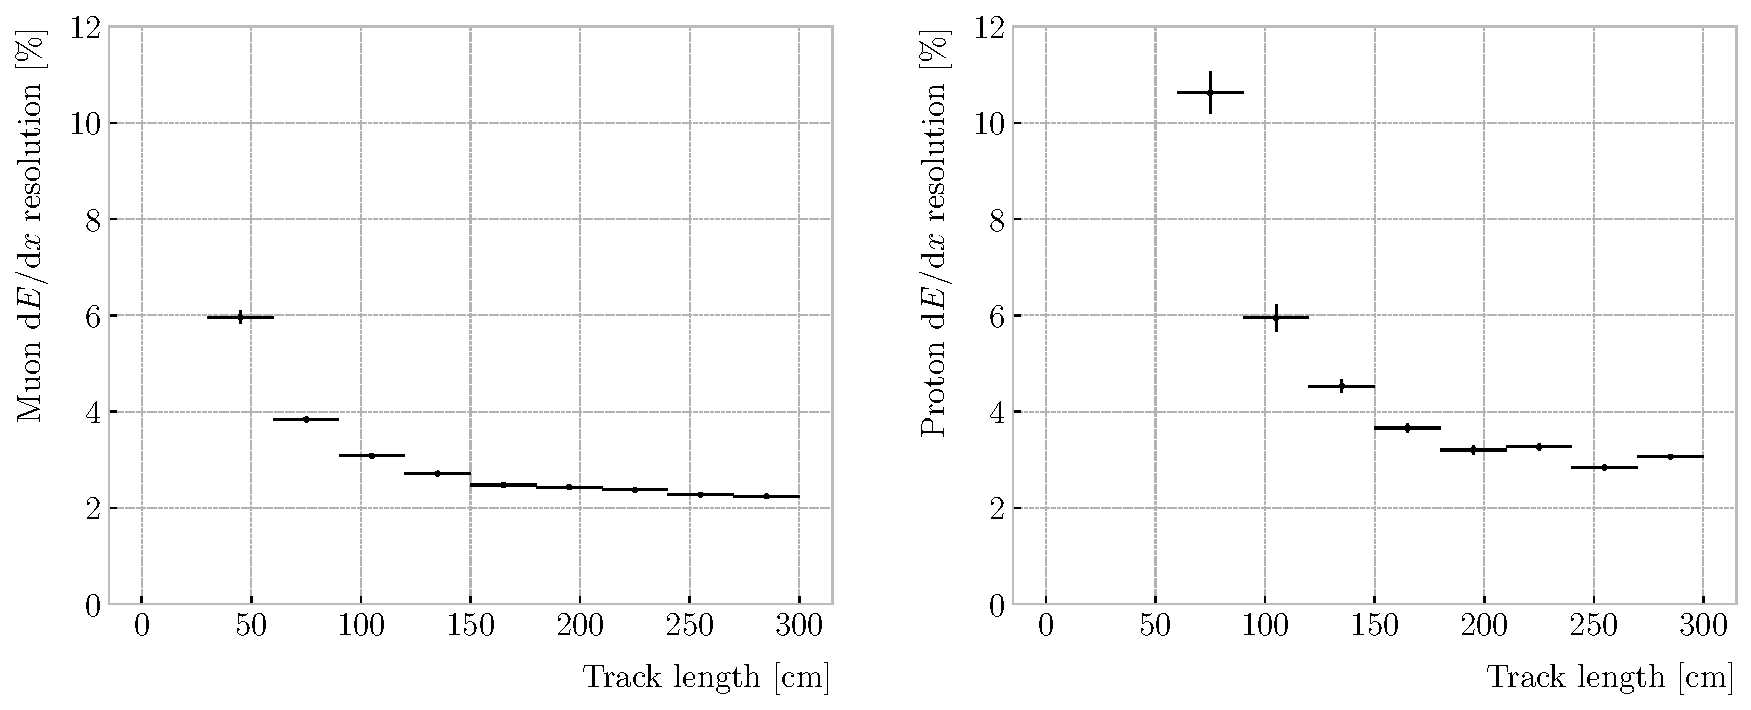
\includegraphics[width=.90\linewidth]{Images/GAr_selection/length_dEdx_resolution_vs_length.pdf}
    \caption[Estimated $\mathrm{d}E/\mathrm{d}x$ resolution as a function of the track length for true muons and protons in a $\nu_{\mu}$ CC sample.]{Estimated $\mathrm{d}E/\mathrm{d}x$ resolution as a function of the track length for true muons (left panel) and protons (right panel) in a $\nu_{\mu}$ CC sample.}
    \label{fig:dEdx_resolution_vs_length}
\end{figure}

% Energy resolution
In terms of the ionisation measurement, both the experience from ALICE and PEP-4 are relevant, as this depends on the readout and the running conditions (pressure and gas mixture). They obtained resolutions of $4.5\%$ and $3.0\%$ for typical track lengths of $160$ and $75~\mathrm{cm}$, respectively. According to previous studies on the $\mathrm{d}E/\mathrm{d}x$ resolution in gaseous detectors \cite{Lehraus1983}, ND-GAr can achieve a $2\%$ resolution for a typical track length of $200~\mathrm{cm}$. Figure \ref{fig:dEdx_resolution_vs_length} shows the values of the resolution I estimate for muons (left panel) and proton (right panel) tracks with different lengths, using the procedure described in section \ref{section:dEdx}.

% Tracking studies
The tracking capabilities of ND-GAr were studied in the context of $\nu_{\mu}$ CC interactions. Using a sample of reconstructed tracks from true muons and charged pions, the tracking efficiency was estimated to be above $90\%$ for momenta $\geq 40 ~ \mathrm{MeV}/c$, with it steadily rising with the momentum. As a function of the angle with respect to the beam direction, the efficiency was almost flat for particles with $p\geq 200 ~ \mathrm{MeV}/c$. In the case of protons, the tracking performs well for kinetic energies $\geq 20 ~ \mathrm{MeV}$. A machine learning algorithm is being developed for low energy proton track identification near the interaction vertex. Preliminary results show an efficiency of $30\%$ at $5 ~ \mathrm{MeV}$ for this method.

% Momentum resolution
The same samples used for the tracking studies were employed to estimate the momentum resolution. The momentum is computed from the curvature of the tracks in the magnetic field, and is therefore limited by the track length in the direction perpendicular to the field. Focusing on the tracks associated to true muons, a double Gaussian fit reveled a width of $2.7\%$ and $12\%$ for the core and tails of the momentum distribution. This same study determined the 3D angular resolution in the HPgTPC to be $0.80^{\circ}$.

The main source of uncertainty in the momentum measurement is the value of the magnetic field. The magnetic field simulations indicate that the overall uncertainty on the central field value is $< 0.05 \%$. A preliminary study investigated the use of $K_{s}^{0}$ decays in the HPgTPC to measure any deviations of the magnetic field from its nominal $0.5 ~ \mathrm{T}$ value. This showed that even a magnetic field bias of $1\%$ will shift the reconstructed invariant mass distribution significantly.

% ECal performance
The results presented for the ECal in Ref. \cite{DUNE2021NDCDR} use an outdated version of the geometry, where the entire ECal sits outside of the pressure vessel and the layers consist of $5~\mathrm{mm}$ of scintillator and $2~\mathrm{mm}$ of Cu. The sample used consists of single photons in a $20^{\circ}$ cone aligned with the beam direction. In the simulation, an energy threshold of $200~\mathrm{keV}$ and a time resolution of $0.25~\mathrm{ns}$ are assumed.

\begin{table}[t]
	\caption[Expected performance for ND-GAr, both from simulation studies and extrapolated from ALICE and PEP-4.]{Expected performance for ND-GAr, both from simulation studies and extrapolated from ALICE and PEP-4. Table adapted from Ref. \cite{DUNE2021NDCDR}.}
	\begin{center}
		\begin{small}
            \begin{tabular}{l|l}
                Parameter                            & Value                                        \\[2mm] \hline
                \rule{0pt}{1.1\normalbaselineskip}Perpendicular hit resolution         & $0.25~\mathrm{mm}$                           \\[2mm] 
                Parallel hit resolution              & $1.50~\mathrm{mm}$                           \\[2mm] 
                Two-track separation                 & $1.00~\mathrm{cm}$                           \\[2mm] 
                $\mathrm{d}E/\mathrm{d}x$ resolution & $5\%$ for protons, $2\%$ for muons           \\[2mm] 
                Tracking efficiency                  & $>90\%$ for $40 ~ \mathrm{MeV}/c$            \\[2mm] 
                Momentum resolution                  & $2.7\%$ core, $12\%$ tails                   \\[2mm] 
                Angular resolution                   & $0.80^{\circ}$                               \\[2mm] 
                Proton detection threshold           & $5 ~ \mathrm{MeV}$                           \\[2mm] 
                ECal energy resolution               & $6\% / \sqrt{E} \oplus 1.6\% / E \oplus 4\%$ \\[2mm] 
                ECal pointing resolution             & $8.17^{\circ} / \sqrt{E} + 4.18^{\circ}$    
            \end{tabular}
		\end{small}
	\end{center}
	\label{tab:detector_systs}
\end{table}

The energy resolution of the photons is obtained from a Gaussian fit. The resulting resolutions are then fitted to a function of the form:
\begin{equation}
    \frac{\sigma_{E}}{E} = \frac{A}{\sqrt{E}} \oplus \frac{B}{E} \oplus C,
\end{equation}
where $A$ is the stochastic term, $B$ the noise term and $C$ the constant term. The best fit finds the values $A=6.1\%$, $B=1.6\%$, and $C=4.5\%$. The photon angle is estimated using a PCA analysis of the associated ECal cluster, taken to be the direction of the first principal component. The angular resolution is computed from a Gaussian fit to the core of the distribution. As a function of the photon energy, the values obtained are $\frac{8.17^{\circ}}{\sqrt{E}} + 4.18^{\circ}$. Different arrangements of the layers and alternative absorber choices may improve these results.

Table \ref{tab:detector_systs} summarises the different detector effects discussed above and the performance expected for ND-GAr.